\documentclass[a4paper]{article}
\usepackage{referencedoc}
\usepackage{tikz}
\usepackage{pgf}
\usetikzlibrary{arrows,automata}
\usepackage{comment}

\title{: \\ }
\author{
  Leonardo \bsc{Moros} \\
  \and
  Guillaume \bsc{Pérution-Kihli} \\
  \and
  Romain \bsc{Ricalens} \\
  \and
  Julien \bsc{Rodriguez} \\
  \and
  Rami \bsc{Younes} \\}
\begin{document}
    \begin{titlepage}
      \begin{sffamily}
            \begin{center}
                \includegraphics[scale=0.6]{pictures/logo_um.png} \\[1cm]
                \textsc{\Large Rapport de projet TER }\\[1cm]
                    
                \HRule \\[0.4cm]{ \huge \bfseries Suppression des redondances dans les bases de connaissances\\[0.4cm] }
                \HRule \\[1.5cm]
                
                \includegraphics[width=\textwidth]{pictures/websem2018-1072x368px.png}
                \\[1.5cm]
                    
                \begin{minipage}{0.4\textwidth}
                    \begin{flushleft} \large
                        Leonardo \bsc{Moros} \\
                          Guillaume \bsc{Pérution-Kihli} \\
                          Romain \bsc{Ricalens} \\
                          Julien \bsc{Rodriguez} \\
                          Rami \bsc{Younes} 
                    \end{flushleft}
                \end{minipage}
                \begin{minipage}{0.4\textwidth}
                    \begin{flushright} \large
                        \emph{Encadrants :} \\ Michel \bsc{Leclère} \\ Marie-Laure \bsc{Mugnier} \\ Federico \bsc{Ulliana}
                    \end{flushright}
                \end{minipage}
                    
                \vfill
                {\large \today}
            \end{center}
      \end{sffamily}
    \end{titlepage}
\newpage
\renewcommand{\contentsname}{Sommaire}
\tableofcontents
\newpage

\section{Introduction}

Une base de connaissances a pour but de regrouper les connaissances d'un domaine spécifique et de les rendre exploitables par un ordinateur. Elle est généralement composée d'une base de faits, qui représente un ensemble de connaissances considérées comme vraies, et d'une base de règles (aussi appelée ontologie) qui permettent de faire des inférences à partir des faits à l'aide d'un moteur d'inférence.
\par Prenons pour exemple une base de connaissances contenant une base de faits avec un seul fait : "Socrate est un humain". Et une base de règles avec une seule règle : "Si X est un humain, alors X est mortel". 
\par Il est possible d'inférer des faits nouveaux. Dans notre exemple, on peut inférer "Socrate est mortel" à partir du fait et de la règle existants. On ajoute ce fait à notre base de faits et on constate qu'on ne peut plus rien inférer de nouveau : on a saturé la base de faits. Ce que l'on vient de faire s'appelle du chaînage avant : on ajoute des nouveaux faits à la base de faits en les inférant à partir des faits existants et des règles, jusqu'à qu'on ne puisse plus rien inférer de nouveau. 
\par Le plus souvent, une base de faits ne contient que des constantes, mais on peut aussi vouloir y intégrer des variables quantifiées existentiellement pour représenter des individus dont on sait qu'ils existent mais dont on ne connaît pas le nom. Et on peut également permettre d'inférer des faits sur des individus qu'on ne connaît pas grâce à ce qu'on appelle une règle existentielle. Par exemple, on peut créer la règle "Si X est humain, alors il existe un Y tel que X a un parent Y".
\par Mais ce type de règle peut être à l'origine de ce qu'on appelle des redondances. Par exemple, ajoutons la règle "Si X est un humain, alors il existe un Y et un Z tels que X a un parent Y et X a un parent Z" à note base de règles. On va pouvoir inférer à partir de "Socrate est un humain", que "il existe un Y tel que Socrate a un parent Y" et "il existe un Z tel que Socrate a un parent Z". Mais ces deux faits sont redondants, on a deux fois l'information qu'il existe un individu qui est parent de Socrate.
\par Les redondances qui peuvent être produites par les règles existentielles, en plus d'ajouter des faits inutiles à la base de faits, peuvent être à l'origine d'une augmentation importante du temps d'exécution nécessaire pour saturer une base de faits. Les faits redondants qui ont été produits peuvent en effet entraîner de nouvelles applications de règles qui peuvent elles-mêmes créer de nouvelles redondances, et ainsi de suite.
\par L'objectif de ce projet de TER est de travailler à la suppression de deux types de redondances : les redondances créées lors de l'exécution d'un algorithme de chaînage avant (suppression dynamique) et les redondances dans les bases de règles (suppression statique).
\par Nous avons donc étudié puis implémenté plusieurs algorithmes de chaînage avant dans Graal\footnote{\url{https://graphik-team.github.io/graal/}}, une bibliothèque réalisée par l'équipe GraphiK\footnote{\url{https://www.lirmm.fr/recherche/equipes/graphik}}. Et nous avons étudié puis implémenté des algorithmes de suppression de redondances dans les bases de règles.

\par Avant d'entrer dans le vif du sujet, il est nécessaire de définir certaines notions essentielles à la compréhension du sujet (section \ref{sec:preliminaires}). Puis, on présentera des algorithmes de chaînage avant ayant différentes propriétés en terme de suppression de redondances et de vitesse de calcul (section \ref{sec:types_de_chases}) afin d'ensuite pouvoir les implémenter (section \ref{sec:conception_implementation}). Ces implémentations ont permis de réaliser des expérimentations pour tester les propriétés de ces algorithmes (section \ref{sec:experimentation}). Enfin, on abordera la suppression des redondances dans les bases de règles (section \ref{sec:regles}).

% \par Notre travail a consisté à utiliser la bibliothèque Graal\footnote{\url{https://graphik-team.github.io/graal/}}, réalisée par l'équipe GraphiK\footnote{\url{https://www.lirmm.fr/recherche/equipes/graphik}}, pour implémenter plusieurs types de chaînages avant (section \ref{sec:conception_implementation}). ) ayant différentes propriétés concernant les redondances qu'ils évitent de créer (section \ref{sec:types_de_chases}). Et également à étudier les redondances au sein des règles pour pouvoir créer une application prenant une base de règles en entrée et retournant une base de règles sans redondance (section \ref{sec:regles}) - toujours en utilisant Graal.
% \par Enfin, des expérimentations ont été réalisées afin de comparer les différents types de chaînages avant en terme de vitesse d'exécution et de capacité à éviter les redondances (section \ref{sec:experimentation}), ainsi que des expérimentations servant à tester l'application supprimant les redondances dans les règles.

%\par Pour commencer, on introduit plus formellement les notions de base concernant les bases de connaissances (section \ref{sec:preliminaires}), puis on détaille les différents types de chaînage avant  pour ensuite expliquer le travail de conception et implémentation que nous avons effectué (section \ref{sec:conception_implementation}) et les expérimentations réalisées (section \ref{sec:experimentation}). Enfin, on explique le travail effectué pour la suppression des redondances dans les règles .
\newpage
\section{Préliminaires}\label{sec:preliminaires}

Les bases de connaissances sont représentées à l'aide de la logique du premier ordre sans les symboles fonctionnels (les objets ne construits que sur des prédicats, des constantes (que l'on notera en minuscule) et des variables (qui commenceront par une majuscule)). Le vocabulaire logique utilisé est composé d'un ensemble fini de prédicats et d'un ensemble infini de constantes. Un atome est de la forme $r(t_1, \ldots, t_n)$ où $r$ est un prédicat d'arité $n$ et les $t_i$ sont des termes. Les conjonctions d'atomes seront représentés par des ensembles d'atomes pour des raisons pratiques.

\begin{definition}[Homomorphisme d'un ensemble d'atomes dans un autre]
Si on voit les ensembles d'atomes comme une conjonction d'atomes fermée existentiellement, alors $S$ s'envoie par homomorphisme dans $S'$ si et seulement si $S$ est conséquence logique de $S'$. Ceci explique pourquoi l'homomorphisme est la notion fondamentale pour le cadre que nous étudions. En particulier deux ensembles d'atomes sont équivalents si chacun s'envoie dans l'autre par homomorphisme. Ici, on le note $A \mapsto B$.
\end{definition}

%\paragraph{Représentation d'un ensemble d'atomes par un graphe} 
On peut représenter un ensemble d'atomes sous la forme d'un graphe biparti d'incidence. Dans ce cas, on a deux types de sommets : des sommets représentant les termes et des sommets représentant les atomes. Ces derniers sont connectés aux premiers par des arêtes numérotées représentant la position du terme dans un atome.
\par Prenons par exemple l'ensemble d'atomes $A = \{p(a,b,X), q(b,X), p(X,Y,a)\}$. On peut la représenter sous la forme du graphe biparti d'incidence suivant : \par

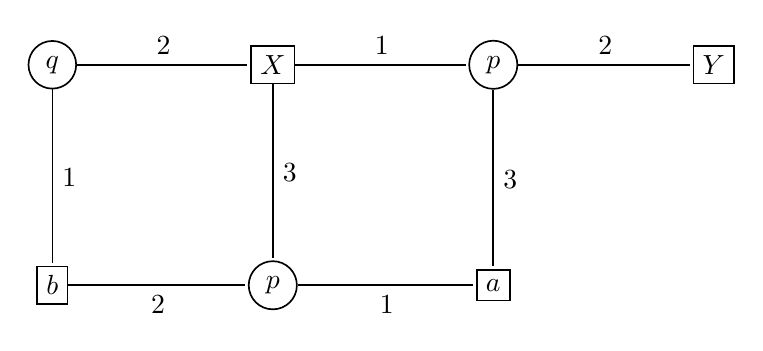
\begin{tikzpicture}[-,>=stealth',shorten >=1pt,auto,node distance=2.8cm,
                    semithick]
  \tikzstyle{every state}=[text=black,minimum size=0.1cm]

  \node[state] [circle]			    (A)                   {$q$};
  \node[state] [rectangle]		   	(B) [right of=A]      {$X$};
  \node[state] [circle]			    (C) [right of=B]      {$p$};
  \node[state] [rectangle]			(D) [right of=C]      {$Y$};
  \node[state] [rectangle]			(E) [below of=A]      {$b$};
  \node[state] [circle]		   	    (F) [below of=B]      {$p$};
  \node[state] [rectangle]			(G) [below of=C]      {$a$};

  \path (A) edge            		node 		        {$2$} 	(B)
            edge            		node                {$1$} 	(E)
        (B) edge            		node        		{$1$} 	(C)
            edge                    node                {$3$} 	(F)
        (C) edge            		node        		{$2$} 	(D)
            edge            		node                {$3$} 	(G)
        (E) edge            		node [below]		{$2$} 	(F)
        (F) edge            		node [below]        {$1$} 	(G);
\end{tikzpicture}

\par Lorsque l'ensemble d'atomes ne contient que des atomes d'arité 2, il est possible de la représenter sous la forme d'un graphe orienté où les sommets représentent les termes et les arcs représentent les atomes.
Soit l'ensemble d'atomes $B = \{p(a,X), q(X,a), p(X,Y)\}$. On peut la représenter par : \par

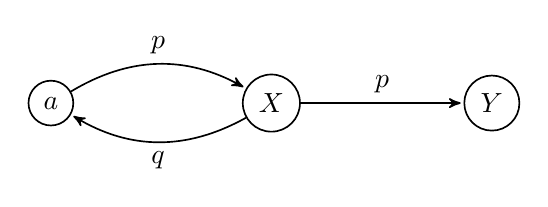
\begin{tikzpicture}[->,>=stealth',shorten >=1pt,auto,node distance=2.8cm,
                    semithick]
  \tikzstyle{every state}=[circle,text=black,minimum size=0.1cm]

  \node[state] 						(A)                   {$a$};
  \node[state]      			   	(B) [right of=A]      {$X$};
  \node[state]         				(C) [right of=B]      {$Y$};

  \path (A) edge [bend left]		node 		        {$p$} 	(B)
        (B) edge [bend left]		node [below]        {$q$} 	(A)
            edge            		node        		{$p$} 	(C);
\end{tikzpicture}


\par Dans la suite du document, toutes ces représentations pourront être utilisées en fonction de leur pertinence dans le contexte.


\begin{definition}[Base de faits] Il s'agit d'un ensemble fini d'atomes. Habituellement, un fait est un atome instancié (c'est-à-dire ne comportant que des constantes) mais on peut admettre des valeurs inconnues dans les bases de faits, auquel cas les atomes peuvent comporter des variables, qui sont quantifiées existentiellement au niveau global (cad : $\{p(a,x), p(x,b)\}$ se traduit en logique par $\exists x (p(a,x) \land p(x,b))$).
\end{definition}

Une règle Datalog est une règle de la forme $body \rightarrow head$ où le corps \textit{(body)} et la tête \textit{(head)} sont des conjonctions d'atomes et toutes les variables apparaissant dans la tête apparaissent aussi dans le corps.
Une règle existentielle est une règle de la forme $body \rightarrow head$ où le corps et la tête sont des conjonctions d'atomes et dont les variables de la tête peuvent être quantifiées existentiellement.

\begin{definition}[Base de connaissances]
Une base de connaissances $\mathcal{K} = (\mathcal{F}, \mathcal{R})$ est composée d'un ensemble de règles existentielles $\mathcal{R}$ et d'une base de faits $\mathcal{F}$.
\end{definition}

Le chaînage en avant, aussi appelée \textit{chase}, est un mécanisme qui enrichit la base de faits en effectuant des applications de règles tant que possible. Un chaînage avant ne termine pas forcément.
Il existe différentes variantes de \textit{chase}, qui diffèrent dans leur pouvoir d'élimination des redondances dans une base de faits en cours de saturation par les règles.
\par On dit qu'une base de faits est saturée lorsque le chaînage en avant ne produit plus de nouveaux faits.


% \begin{definition}[Homomorphisme, noté $\mapsto$]
% Soit deux ensembles d'atomes $F$ et $G$. Un homomorphisme $h$ de $F$ dans $G$ est une substitution des variables de $F$ par des termes de $G$, telle que pour tout atome $p(t_1, \ldots, t_n) \in F$, $p(h(t_1), \ldots, h(t_n)) \in G$.
% \end{definition}

% \begin{definition}[Homomorphiquement équivalent]
% Deux ensembles d'atomes $F$ et $G$ sont homomorphiquement équivalents si il existe des homomorphismes $h : F \mapsto G$ et $h' : G \mapsto F$. Ils sont isomorphes si ces homomorphismes sont bijectifs.
% \end{definition}

% \begin{example} 
% Soit A et B deux ensembles d'atomes tel que $A={p(a,b), p(b,X1)}$ et $B={p(a,b), p(b,Y1), p(b,Z1)}$
% On a A et B homomorphiquement équivalents mais non isomorphiquement équivalents.
% \end{example}


\begin{definition}[Redondance dans un ensemble d'atomes]
Un ensemble d'atomes S est redondant s'il existe un homomorphisme de S dans l'un de ses sous-ensembles stricts.
\end{definition}

\begin{definition}[Core]\label{def:Core}
Un core est un ensemble d'atomes non redondant.
\par Le core d'un ensemble d'atomes S est un sous-ensemble de S équivalent à S. S peut avoir plusieurs cores, mais dans ce cas ils sont tous isomorphes (on passe de l'un à l'autre par un renommage bijectif des variables), c'est pourquoi on s'autorise à dire "le core" de S.
\end{definition}

% \begin{definition}[Sous-graphe induit]
% Soit un graphe $G = (V,E)$ et $S$ un sous-ensemble de $V$. Un sous-graphe induit de $G$ est un sous-graphe dont l'ensemble des sommets est $S$ et dont les arêtes sont toutes les arêtes de $E$ qui relient entre eux deux sommets inclus dans $S$.
% \end{definition}

%\begin{definition}[Gel de variables]
Le \textit{Freeze} ou gel d'une variable est le fait de substituer une constante pas encore utilisée \textit{(fresh constant)} à cette variable.
%\end{definition}

\paragraph{Notation}\label{def:freeze()} On notera $freeze(A)$ la procédure prenant en paramètre l'ensemble d'atomes $A$ et renvoyant cet ensemble avec ses variables gelées. Et on notera $freeze(A,B)$ la procédure prenant en paramètre deux ensembles d'atomes $A$ et $B$ et renvoyant l'union de ces deux ensembles avec uniquement les variables de A gelées (ce qui comprend le gel des variables dans $B$ qui sont aussi contenues dans $A$).
% \begin{definition}[Gel d'atomes]
% Le \textit{Freeze} ou gel d'un atome est le fait de substituer à chacune de ces variables une constante pas encore utilisé \textit{(fresh constant)}.
% \end{definition}

% \begin{proposition}
% Le \textit{core} $C$ d'un graphe $G$ est toujours un sous-graphe induit de $G$.
% \end{proposition}

% Preuve à ré-écrire
% \begin{proof}
%     Puisque $C$ est le \textit{core} de $G$, alors, par définition, il existe un homomorphisme $h : C \mapsto G$. Cela veut donc dire que chaque sommet de $C$ doit pouvoir s'envoyer sur un sommet $G$ et puisque $C$ est de taille minimale par définition, aucun sommet de $C$ ne va s'envoyer sur un même sommet de $G$ (sinon, $C$ ne serait pas un \textit{core}). En conséquence, $C$ est un sous-graphe induit de $G$.
% \end{proof}

\begin{definition}[Pièce d'un ensemble d'atomes / d'une base de faits]\label{def:piece_atomes}
    On appelle pièce d’un ensemble d'atomes $A$ un sous-ensemble $P$ non vide d’atomes qui vérifie : 
    \begin{itemize}
        \item pour toute variable existentielle $z$ de l'ensemble d'atomes $A$, si un atome contenant $z$ est dans $P$ alors tous les atomes qui contiennent $z$ sont dans $P$ 
        \item $P$ est minimal pour cette propriété.
    \end{itemize}
\end{definition}



% \begin{definition}[Logique du premier ordre]
% (à reprendre).
% calcul des prédicats du premier ordre, ou calcul des relations prend la forme de prédicats explicitant les relations entre les différentes variables d'un problème par des connecteurs logiques et les quantificateurs existentiel et universel.
% \par Un terme est une constante ou une variable. Un atome est de la forme $r(t_1, \ldots, t_n)$ où $r$ est un prédicat d'arité $n$ et les $t_i$ sont des termes.
% \end{definition}

% \begin{definition}[Fragment conjonctif positif existentiel de la logique du premier ordre]
% (À faire)
% \end{definition}

% le Datalog est un langage de programmation logique ayant une syntaxe particulière dont nous nous sommes servis pour la notation de nos règles.

% \begin{definition}[Requête]
% Soit une base de connaissances $\mathcal{K} = (\mathcal{F}, \mathcal{R})$. L'interrogation de la base en posant une requête $\mathcal{Q}$ définit la conséquence logique suivante : $\mathcal{F}, \mathcal{R} \vDash \mathcal{Q}$.
% \end{definition}
\newpage
\section{Le chaînage avant (\textit{chase})}\label{sec:types_de_chases}

% Le chaînage avant est une stratégie de calcul des réponses à une requête $\mathcal{Q}$. On part du corps d'une règle pour déduire de nouveaux faits présent dans la tête de la règle. Le chaînage avant peut s'appliquer en largeur et en profondeur.

Dans cette partie différents types de chaînages avant vont être présentés. Tout d'abord, il faut distinguer le chaînage en avant en profondeur de celui en largeur : en largeur, on applique chaque règle à partir d'une base de faits $\mathcal{F}_i$ pour obtenir une base de faits $\mathcal{F}_{i+1}$ à partir de laquelle on ré-applique les règles, et ainsi de suite jusqu'à saturation. En profondeur, on applique les règles sur la même base de faits jusqu'à saturation. Dans le cadre de ce projet, on ne s'intéresse qu'au chaînage en avant en largeur.
\par Mais avant de présenter différentes variantes du chaînage avant en largeur, nous devons construire une base commune à tous ces $chases$ en vue notamment de leur implémentation future. Ainsi, on présente un algorithme de chaînage avant suffisamment générique (section \ref{subsec:algo_base_ch_avant}) pour qu'il soit la base de tous les types de chaînages en avant que nous allons présenter  (section \ref{subsec:types_chases}).

% \begin{definition}[chaînage avant en largeur]
% A chaque itération du chaînage avant, toutes les règles candidates sont déclenchées.
% \end{definition}

% \begin{definition}[chaînage avant en profondeur]
% A chaque itération du chaînage avant, seule la première règle candidate est déclenchée.
% \end{definition}

% \begin{definition}[Saturation d'une base de faits]
% Soit une base de connaissances $\mathcal{K} = (\mathcal{F}, \mathcal{R})$. Saturer $\mathcal{F}$
% consiste à calculer la base de faits saturée $\mathcal{F^*}$ obtenue en appliquant de manière itérative les règles de $\mathcal{R}$ sur $\mathcal{F}$ jusqu'à stabilité (on ne déduit pas de nouveaux faits).   
% \end{definition}

%\begin{definition}[Saturation finie/infinie]
%\par On dit que si la saturation $\mathcal{F}^*$ est finie alors il existe $k \in \mathbb{N}$ borné tel que $\mathcal{F}_k$ = $\mathcal{F^*}$.
%De même on dit que si la saturation $\mathcal{F^*}$ est infinie alors il n'existe pas de borne pour un tel $k$.   
%\end{definition}

% \begin{definition}[Modèle universel]
% Si il existe un modèle universel $\mathcal{M}$ pour une base de connaissance $\mathcal{K}$ alors, tout modèle $\mathcal{M}_i$ de $\mathcal{K}$ admet un homomorphisme $h$ tel que $h(\mathcal{M}_i)$ = $\mathcal{M}$.   

%\end{definition}

\subsection{Algorithme de base}\label{subsec:algo_base_ch_avant}

Commençons tout d'abord par définir la notion de déclencheur (ou \textit{trigger}) : il s'agit d'un couple $(R = B \rightarrow H,h)$ où $R$ est une règle et $h$ un homomorphisme permettant d'envoyer $B$, le corps de la règle $R$, sur la base de faits.
\par Un déclencheur est dit nouveau si il n'a pas été trouvé lors d'une étape précédente du chaînage avant en largeur.
\par Il est dit applicable si il respecte le critère d'applicabilité, qui diffère en fonction du type de chaînage en avant. La variation du critère d'applicabilité d'une règle n'a d'intérêt que pour les règles existentielles. En effet, avec les règles Datalog, les chaînages avant s'arrêtent toujours tandis que l'arrêt avec les règles existentielles varie en fonction des critères d'applicabilité des règles utilisés.
\par Une extension locale est un algorithme qui prend en paramètre les nouveau faits de l'étape en cours et un déclencheur applicable et qui produit des nouveaux faits à partir du déclencheur pour les ajouter aux nouveaux faits de l'étape en cours - cet algorithme varie en fonction du type de \textit{chase}.
\par Une extension globale est un algorithme prenant en paramètre la base de faits de l'étape précédente et les nouveaux faits de l'étape en cours et qui produit la base de faits de l'étape en cours - il varie lui aussi en fonction du type de \textit{chase}.
\par Ceci posé, on peut décrire notre algorithme de chainage avant en largeur.

\begin{definition}[Chaînage avant en largeur]
Soit une base de connaissances $\mathcal{KB} = (\mathcal{F}_0, \mathcal{R})$. Un chaînage avant en largeur consiste, à partir d'une base de faits $\mathcal{F}_i$ à générer une base de faits $\mathcal{F}_{i+1}$ en :
\begin{itemize}
    \item Ajoutant le contenu de $\mathcal{F}_{i}$ à $\mathcal{F}_{i+1}$ .
    \item Pour chaque règle $R = B \rightarrow H \in \mathcal{R}$, trouver tous les nouveaux déclencheurs $(R,h(B))$ tels que $h(B) \vDash \mathcal{F}_i$ 
    \item Tester si le déclencheur $(R,h(B))$ est applicable, et si il l'est, faire une extension locale des nouveaux faits $h(H)$.
    \item Une fois toutes les règles appliquées, réaliser l'extension globale.
\end{itemize}
\end{definition}

\par
L'algorithme \ref{algo:chainage_avant_largeur} présente un chaînage avant en largeur général.
% \par De même, l'algorithme \ref{algo:chainage_avant_largeur} n'explique comment la base de faits est étendue à chaque étape, cela est précisé dans l'algorithme \ref{algo:etendre_general} pour tous les chaînages avant à l'exception de certains comme le \textit{core chase} qui a sa propre méthode d'extension de la base de faits.
% \par De même, lors de chaque application de règle, il y a une extension dite locale consistant à sélectionner les nouveaux faits qui seront fournis à l'extension globale. La version par défaut est l'algorithme \ref{algo:etendre_local_defaut}.

%\paragraph{Homomorphisme sûr} Un homomorphisme $h^s$ est une extension d'un homomorphisme $h$ consistant à remplacer les variables de l'ensemble d'atomes sur lequel est appliqué $h^s$ par des noms de variables "frais", autrement dit des noms de variables n'existant pas encore dans la base de faits que l'on sature.
%\newline

\setstretch{1}
\begin{algorithm}[H]\label{algo:chainage_avant_largeur}
\caption{Chaînage avant en largeur}
\SetAlgoLined
\DontPrintSemicolon

\SetKwInOut{Input}{entrées}
\SetKwInOut{Output}{sortie}
\Input{une base de faits $\mathcal{F}$, une base de règles $\mathcal{R}$}
\Output{la base de faits saturée $\mathcal{F^*}$}
\SetKwRepeat{Do}{faire}{tant que}

$\mathcal{F}_0 \gets \mathcal{F}$\;
$n \gets 0$\;

\Do{$nouvFait \not= \emptyset$}
{
    $nouvFaits\gets \emptyset$ \;
    \ForEach{règle : $ R = B \rightarrow  H \in \mathcal{R}$} 
    {
        \ForEach{nouveau déclencheur $(R,h)$ tel que $h : B \mapsto \mathcal{F}_n$} 
        {
            \uIf{$estApplicable(R,h)$}
            {
                $nouvFaits \leftarrow \mbox{\textit{étendreLocalement}}(nouvFaits, (R,h))$\;
            }
        }
    }
    $\mathcal{F}_{n+1} \gets \mbox{\textit{étendreLocalement}}(\mathcal{F}_{n}, nouvFaits)$\;
    $n \gets n + 1$\;
}
\Return $\mathcal{F}_n$
\end{algorithm}
\setstretch{1.5}

% \paragraph{}
% L'algorithme de chaînage avant est une application itérative de règles, à chaque étape on applique chaque règle respectant les contraintes et on continue à la prochaine étape jusqu'à ce qu'il n'y ait plus des règles applicables. Il est important de remarquer que si une règle est applicable à l'étape $I_n$ par rapport à un homomorphisme $h$ elle sera aussi applicable à l'étape $I_{n+1}$. Pour éviter cette situation qui nous emmènerait à boucler à l'infini l'algorithme de chaînage avant n'applique une règle $R$ par rapport à un homomorphisme $h$ qu'une seule fois.\newline

Pour les extensions globales et locales, il est possible d'écrire des algorithmes génériques qui conviendront à la plupart des types de chaînage avant qui vont être présentés, à quelques exceptions près. On fournit donc un algorithme d'extension locale par défaut (algorithme \ref{algo:etendre_local_defaut}) et un algorithme d'extension globale par défaut (algorithme \ref{algo:etendre_general}).
\par Pour l'algorithme d'extension locale, il convient d'expliquer comment on obtient les nouveaux faits à partir d'un déclencheur. Soit une règle $R = B \rightarrow H$ et un déclencheur applicable $(R,h)$ tel que $h : B \mapsto \mathcal{F}$ où $\mathcal{F}$ est la base de faits. Les nouveaux faits sont le résultat de $h^{safe}(H)$ où $h^{safe}$ est une substitution obtenue à partir de $h$ où chaque variable de $H$ qui n'est pas remplacée dans $h$ est remplacée par une variable fraîche, c'est-à-dire une variable qui n'a pas encore été utilisée dans la base de faits.


\setstretch{1}
\begin{algorithm}[H]\label{algo:etendre_local_defaut}
\caption{étendreLocalement (par défaut)}
\SetAlgoLined
\DontPrintSemicolon
\SetKwInOut{Input}{entrées}
\SetKwInOut{Output}{sortie}
\Input{
   $nouvFaits$ : les nouveaux faits de l'étape en cours
    \par $(R = B \rightarrow H,h)$ : le déclencheur à appliquer}
\Output{l'extension de $nouvFaits$}
    \Return $nouvFaits \cup h^{safe}(H)$\;
\end{algorithm}
\setstretch{1.5}

\setstretch{1}
\begin{algorithm}[H]\label{algo:etendre_general}
\caption{étendreGlobalement (par défaut)}
\SetAlgoLined
\DontPrintSemicolon
\SetKwInOut{Input}{entrées}
\SetKwInOut{Output}{sortie}
\Input{une base de faits $\mathcal{F}$, une liste de faits $nouvFaits$}
\Output{la base de faits $\mathcal{F'}$ étendue}
    $\mathcal{F'} \gets \mathcal{F} \cup nouvFaits$\;
    \Return $\mathcal{F'}$
\end{algorithm}
\setstretch{1.5}

Maintenant que la base commune aux différents types de \textit{chase} a été posée, on va pouvoir les présenter.

\subsection{Types de \textit{chases}}\label{subsec:types_chases}

Cette partie a pour objet de présenter tous les chases qui ont été implémentés dans le cadre du projet.
\par Quatres de ces chases sont "classiques" dans la littérature scientifique du domaine. Dans l'ordre de leur capacité à éviter les redondances : l'\textit{oblibious chase} (\ref{sec:oblivious_chase}), le \textit{semi-oblivious chase} (\ref{sec:semi_oblivious_chase}), le \textit{restricted chase} (\ref{sec:restricted_chase}) et le \textit{core chase} (\ref{sec:core_chase}). 
\par Deux autres chases, proposés par Stathis Delivorias, un doctorant de l'équipe GraphiK, vont aussi être présentés : le \textit{local core chase} (\ref{sec:local_core_chase}) et le \textit{vacuum chase} (\ref{sec:vacuum_chase}).

\subsubsection{L'Oblivious \textit{chase}}\label{sec:oblivious_chase}

L'\textit{oblivious chase} est le type de chaînage avant générant le plus de redondances. Il ne fait en effet aucun filtre pour les éliminer : un déclencheur est considéré comme étant toujours applicable (algorithme \ref{algo:est_applicable_oblivious}).
\par Ce faisant, ses propriétés d'arrêt sont médiocres sur les règles existentielles, et il est donc facile de trouver des cas où l'algorithme ne s'arrête pas.

\setstretch{1}
\begin{algorithm}[H]\label{algo:est_applicable_oblivious}
\caption{estApplicable (Oblivious)}
\SetAlgoLined
\DontPrintSemicolon
\SetKw{Break}{break}
\SetKwInOut{Input}{entrées}
\SetKwInOut{Output}{sortie}
\Input{Un déclencheur $(R,h)$}
\Output{vrai si le déclencheur $(R,h)$ est applicable}
\Return $vrai$
\end{algorithm}
\setstretch{1.5}

Pour illustrer cet algorithme prenons un exemple où il s'arrête : soit la base de connaissances $\mathcal{KB}_A = (\mathcal{F} = \{p(a,b)\}, \mathcal{R} = \{R = p(x,y) \rightarrow q(x,z) \})$.
\begin{center}
\begin{tabular}{|c|c|}
    \hline
    Étape & Base de faits  \\ 
    \hline
    1 &$\mathcal{F} \cup \{q(a, z_1)\}$ \\ 
    \hline
    2 &$\mathcal{F}_1$  \\
    \hline
\end{tabular}
\end{center}
On constate que l'algorithme s'arrête à la deuxième étape.
\par Prenons un exemple ou l'\textit{oblivious chase} ne s'arrête pas. Soit
$\mathcal{KB}_B = (\mathcal{F} = \{p(a,b)\}, \mathcal{R} = \{R = p(x,y) \rightarrow p(x,z) \})$

\begin{center}
\begin{tabular}{|c|c|}
    \hline
    Étape & Base de faits  \\ 
    \hline
    1 &$\mathcal{F} \cup \{p(a, z_1)\}$ \\ 
    \hline
    2 &$\mathcal{F}_1 \cup \{p(a, z_2)\}$ \\
    \hline
    ... & ... \\
    \hline
    $i+1$ & $\mathcal{F}_i \cup \{p(a, z_{i+1})\} $ \\
    \hline
\end{tabular}
\end{center}

On constate bien que la saturation ne s'arrête jamais : la règle produit un atome redondant qui permet de la ré-appliquer à l'infini. Le \textit{semi-oblivious chase} va permettre d'éviter que l'algorithme ne s'arrête pas dans ce type de cas.

\subsubsection{Le \textit{semi-oblivious chase}}\label{sec:semi_oblivious_chase}

%L'algorithme du Semi-Oblivious \textit{chase} est très proche de l'Oblivious Chase, comme ce dernier il n'applique une règle $R$ par rapport à un homomorphisme $h$ qu'une seule fois, mais en plus il compare aussi les frontières de l'homomorphisme $h$ avec les frontières des éléments de la base de faits. Si il en trouve des identiques alors $h$ n'est pas ajouté à la base de faits.%

% \begin{definition}[Déclencheur]
% Soit une base de connaissances $\mathcal{K} = (\mathcal{F}, \mathcal{R})$ et $R$ une règle tel que $R \in \mathcal{R}$ de la forme $B \rightarrow  H$.
% Un couple $(R,h)$ est un déclencheur pour $\mathcal{F}$ si $h$ est un homomorphisme de $B$ dans $\mathcal{F}$.
% \end{definition}

L'algorithme du Semi-Oblivious \textit{chase} a un critère d'applicabilité plus strict que l'\textit{oblivious chase} (algorithme \ref{algo:est_applicable_semi_oblivious}). En effet, on va stocker les déclencheurs des applications précédentes pour pouvoir les comparer aux déclencheurs en cours d'application.
\par On retient donc une liste $L$ de tous les déclencheurs appliqués précédemment. Lorsque l'on veut tester si un déclencheur $(R,h)$ est applicable, alors on recherche dans $L$ si il existe un déclencheur $(R,g)$ tel que $h(frontier(R)) = g(frontier(R))$. Si c'est le cas, la règle n'est pas applicable, sinon elle l'est.
\par L'idée ici est que, si les substitutions $h$ et $g$ envoient la frontière sur les mêmes variables, alors les atomes produits par $h^{safe}(H)$ seront forcément redondants par rapport à ceux de $g^{safe}(H)$ car ils seront isomorphes.

\begin{proposition}
    Si l'\textit{oblivious chase} s'arrête, alors le \textit{semi-oblivious} s'arrête aussi.
\end{proposition}

\begin{proof} Le \textit{semi-oblivious chase} a une condition sur la frontière en plus il aura donc au pire la même efficacité que l'\textit{oblivious}.
\end{proof}

\setstretch{1}
\begin{algorithm}[H]\label{algo:est_applicable_semi_oblivious}
\caption{estApplicable (Semi-Oblivious)}
\SetAlgoLined
\DontPrintSemicolon
\SetKw{Break}{break}
\SetKwInOut{Input}{entrées}
\SetKwInOut{Output}{sortie}
\Input{$(R,h)$ : le déclencheur à tester
\par $L$ : la liste des déclencheurs précédemment appliqués}
\Output{vrai si le déclencheur $(R,h)$ est applicable, faux sinon}
    \uIf{il existe $(R,g) \in L$ tel que $h(frontier(R)) = g(frontier(R))$}
    {
        \Return faux
    }
\Return $vrai$
\end{algorithm}
\setstretch{1.5}
Illustrons maintenant l'algorithme en reprenant l'exemple où l'\textit{oblivious chase} ne s'arrête pas.
\par Soit $\mathcal{KB}_B = (\mathcal{F} = \{p(a,b)\}, \mathcal{R} = \{R = p(x,y) \rightarrow p(x,z) \})$

\begin{center}
\begin{tabular}{|c|c|c|}
    \hline
    $\mathcal{F}$ & Oblivious & Semi-oblivious \\ 
    \hline
    1 &$\mathcal{F} \cup \{p(a, z_1)\}$ & $\mathcal{F} \cup \{p(a, z_1)\} $\\ 
    \hline
    2 &$\mathcal{F}_1 \cup \{p(a, z_2)\}$ &$\mathcal{F}_1$\\
    \hline
    ... & ... & \\
    \hline
    $i+1$ & $\mathcal{F}_i \cup \{p(a, z_{i+1})\} $& \\
     \hline
     ... & ... & \\
     \hline
\end{tabular}
\end{center}

Ici, le semi-oblivious chase termine la saturation lors de la deuxième étape car le seul nouveau délencheur trouvé $(R,\{x \rightarrow a$, $y \rightarrow z_1\})$ a le même effet sur la frontière (qui ne contient que $x$) que le déclencheur $(R,\{x \rightarrow a$, $y \rightarrow b\})$ appliqué lors de la première étape.  

\par Cependant, c'est un algorithme pour lequel il reste facile de trouver des exemples dans lesquels il ne s'arrête pas.
Soit $\mathcal{KB}_C = (\mathcal{F} = \{p(a,a)\}, \mathcal{R} = \{R = p(x,y) \rightarrow p(y,z) \})$

\begin{center}
\begin{tabular}{|c|c|}
    \hline
    $\mathcal{F}$ & Semi-oblivious \\ 
    \hline
    1  & $\mathcal{F} \cup \{p(a, z_1)\} $ \\ 
    \hline
    2  &$\mathcal{F}_1 \cup \{p(z_1, z_2)\}$  \\
    \hline
    ...  & ...  \\
    \hline
    i+1 & $\mathcal{F}_i \cup \{p(z_{i}, z_{i+1})\} $   \\
     \hline
     ...  & ...  \\
     \hline
\end{tabular}
\end{center}
C'est pour cela que l'on va introduire le \textit{restricted chase}.

\subsubsection{Le \textit{restricted chase}}\label{sec:restricted_chase}

Le \textit{restricted chase} a une approche différente pour éviter les redondances. Pour décider si un déclencheur $(R = B \rightarrow H,h)$ est applicable, on va tester l'existence d'une substitution $h'$ telle que $h \subset h'$ et $h'(H) \in \mathcal{F}$, $\mathcal{F}$ étant la base de faits. Si un tel $h'$ existe, alors on n'applique pas le déclencheur. L'idée ici est que, si $h'$ existe, alors les atomes produits à l'aide de ce déclencheur seront forcément redondants par rapport à la base de faits puisque il existe des atomes équivalents au nom des variables près.
\par Le critère du \textit{restricted chase} est plus puissant que celui du \textit{semi-oblivious chase}. En effet, dans le \textit{semi-oblivious chase}, si il existe un déclencheur ayant le même effet sur la frontière de la règle qu'un déclencheur appliqué précédemment, alors ce déclencheur précédent a produit des atomes qui sont dans la base de faits et par rapport auxquels le nouveau déclencheur produira forcément des atomes redondants, que le critère du \textit{restricted chase} sera en mesure de détecter. Par conséquent, si un \textit{semi-oblivious chase} s'arrête, alors le \textit{restricted chase} s'arrête aussi.
\par Concernant le critère d'applicabilité, il y a deux façons de l'utiliser : soit la base de faits sur laquelle on fait le test est la base de faits courante de l'étape en cours ($\mathcal{F}_n$), et dans ce cas on dira que le \textit{restricted chase} est parallèle (algorithme \ref{algo:est_applicable_restricted_parallel}). Soit il s'agit de base de faits courante à laquelle on ajoute les nouveaux faits produits dans l'étape en cours ($\mathcal{F}_n \cup nouvFaits$) et dans ce cas, on parlera de \textit{restricted chase} en largeur (algorithme \ref{algo:est_applicable_restricted_largeur}).

\setstretch{1}
\begin{algorithm}[H]\label{algo:est_applicable_restricted_parallel}
\caption{estApplicable (\textit{restricted chase} en parallèle)}
\SetAlgoLined
\DontPrintSemicolon
\SetKwInOut{Input}{entrées}
\SetKwInOut{Output}{sortie}
\Input{$(R,h)$ : le déclencheur à tester
\par $\mathcal{F}_n$ : la base de faits courante }
\Output{vrai si le déclencheur $(R,h)$ est applicable, faux sinon}
    \uIf{il existe $h'$ tel que $h \subset h'$ et $h'(H) \in \mathcal{F}$}
    {
        \Return $faux$
    }
\Return $vrai$
\end{algorithm}
\setstretch{1.5}
\setstretch{1}
\begin{algorithm}[H]\label{algo:est_applicable_restricted_largeur}
\caption{estApplicable (\textit{restricted chase} en largeur)}
\SetAlgoLined
\DontPrintSemicolon
\SetKwInOut{Input}{entrées}
\SetKwInOut{Output}{sortie}
\Input{$(R,h)$ : le déclencheur à tester
\par $\mathcal{F}_n$ : la base de faits courante
\par $nouvFaits$ : les nouveaux faits obtenus durant l'étape courante}
\Output{vrai si le déclencheur $(R,h)$ est applicable, faux sinon}
    \uIf{il existe $h'$ tel que $h \subset h'$ et $h'(H) \in \mathcal{F} \cup nouvFaits$}
    {
        \Return $faux$
    }
\Return $vrai$
\end{algorithm}
\setstretch{1.5}

\par La version largeur est susceptible de produire moins de redondances que la version parallèle, car elle peut permettre d'éviter des redondances produites par d'autres règles durant la même étape. Cependant, elle présente le défaut d'être non-déterministe : en effet, le résultat du chaînage avant va différer en fonction de l'ordre d'application des règles, comme cela est illustré dans l'exemple \ref{ex:restricted_largeur_non_deterministe}.

\begin{example}
% oblivious , expl 3
$\mathcal{KB}_C = (\mathcal{F} = \{p(a,a)\}, \mathcal{R} = \{R = p(x,y) \rightarrow p(y,z) \})$

\begin{center}
\begin{tabular}{|c|c|c|c|}
    \hline
    $\mathcal{F}$ & Oblivious & Semi-oblivious & Restricted \\ 
    \hline
    1 &$\mathcal{F} \cup \{p(a, z_1)\}$ & $\mathcal{F} \cup \{p(a, z_1)\} $&  $\mathcal{F}$ \\ 
    \hline
    2 &$\mathcal{F}_1 \cup \{p(z_1, z_2)\}$ &$\mathcal{F}_1 \cup \{p(z_1, z_2)\}$ & \\
    \hline
    ... & ... & ... & \\
    \hline
    i+1 & $\mathcal{F}_i \cup \{p(z_{i}, z_{i+1})\} $& $\mathcal{F}_i \cup \{p(z_{i}, z_{i+1})\} $&   \\
     \hline
     ... & ... & ... & \\
     \hline
\end{tabular}
\end{center}
\end{example}

Ici, le \textit{restricted chase} termine la saturation lors de la première étape étape car le seul homomorphisme trouvé $h = (x \rightarrow a, y \rightarrow a)$ peut être étendu en $h' = (x \rightarrow a, y \rightarrow a, z \rightarrow a)$ tel que $h'(p(y,z)) = p(a,a) \in \mathcal{F}$. 

\begin{example}\label{ex:restricted_largeur_non_deterministe}
% oblivious , expl 4
$\mathcal{KB}_D = (\mathcal{F} = \{p(a,b)\}, \mathcal{R} = \{R_1 = p(x,y) \rightarrow p(y,z) , R_2 = p(x,y) \rightarrow p(y,y) \})$

\begin{center}
% \begin{tabular}{|c|c|c|}
%     \hline
%     $\mathcal{F}$ & Oblivious & Semi-oblivious \\ 
%     \hline
%     1 &$\mathcal{F} \cup \{p(b, z_1), p(b,b)\}$ & $\mathcal{F} \cup \{p(b, z_1), p(b,b)\} $\\ 
%     \hline
%     2 &$\mathcal{F}_1 \cup \{p(z_1, z_2), p(z_1, z_1), p(b, z_3)\}$ &$\mathcal{F}_1 \cup \{p(z_1, z_2), p(z_1, z_1)\}$  \\
%     \hline
%     ... & ... & ...  \\
%     \hline
%     i+1 & $\mathcal{F}_i \cup \{p(z_{i}, z_{i+1}), p(z_{i}, z_{i}), p(z_{i-1}), p(z_{i+2}), ...\} $& $\mathcal{F}_i \cup \{p(z_{i}, z_{i+1}), p(z_{i}, z_{i})\} $ \\
%      \hline
%      ... & ... & ... \\
%      \hline
% \end{tabular}
\begin{tabular}{|c|c|c|c|c|}
    \hline
    $\mathcal{F}$ & \textit{restricted chase} en parallèle & \textit{restricted chase} en largeur ($R_1$ / $R_2$) & \textit{restricted chase} en largeur ($R_2$ / $R_1$)  \\ 
    \hline
    1 &  $\mathcal{F} \cup \{p(b, z_1), p(b,b)\} $ &  $\mathcal{F} \cup \{p(b, z_1), p(b,b)\} $ & $\mathcal{F} \cup \{p(b,b)\}$ \\ 
    \hline
    2 &$\mathcal{F}_1 \cup \{p(z_1, z_2), p(z_1, z_1)\}$ &$\mathcal{F}_1 \cup \{p(z_1, z_2), p(z_1, z_1)\}$& $\mathcal{F}_1$ \\
    \hline
    ... & ... & ... &  \\
    \hline
    i+1 &  $\mathcal{F}_i \cup \{p(z_{i}, z_{i+1}), p(z_{i}, z_{i})\} $   &  $\mathcal{F}_i \cup \{p(z_{i}, z_{i+1}), p(z_{i}, z_{i})\} $  & \\
     \hline
     ... & ... &  ... &  \\
     \hline
\end{tabular}
\end{center}
\end{example}

Dans cet exemple, l'ordre d'application des règles modifie le résultat de la saturation. Lorsque l'on utilise l'ordre $R_1$/$R_2$ la saturation est infinie, alors qu'avec l'ordre $R_2$/$R_1$, la saturation se termine lors de la deuxième étape. Le \textit{restricted chase} en parallèle donne le même résultat que celui en largeur avec l'ordre $R_1$/$R_2$.
\par Cet exemple nous permet aussi de constater que le \textit{restricted chase} est lui-aussi susceptible de produire des redondances et de ne pas s'arrêter pour cette raison. Le type de \textit{chase} qui suit ne produit quant à lui aucune redondance.

\subsubsection{Core chase}\label{sec:core_chase}

Le \textit{core chase} est un chaînage avant qui consiste, lors de chaque étape en largeur, à calculer le \textit{core} de la base faits courante afin de supprimer toute redondance (algorithme \ref{algo:etendre_core_chase}).
Cela a pour conséquence que, si une base de connaissances possède un modèle universel fini, alors le \textit{core chase} s'arrête en un nombre fini d'étapes.
\par Le \textit{core chase} utilise l'applicateur de règles du \textit{restricted chase}. Autant la version parallèle que celle en largeur peuvent être utilisées : en effet, il n'y a pas de problème de résultat modifié par l'ordre d'application des règles puisque toutes les redondances sont supprimées. Le résultat d'une étape sera toujours isomorphe au résultat de la même étape obtenu avec un autre ordre d'application des règles.

\setstretch{1}
\begin{algorithm}[H]\label{algo:etendre_core_chase}
\caption{étendreGlobalement (\textit{core chase})}
\SetAlgoLined
\DontPrintSemicolon
\SetAlgoLined
\DontPrintSemicolon
\SetKwInOut{Input}{entrées}
\SetKwInOut{Output}{sortie}
\Input{$\mathcal{F}$ : la base de faits à étendre
\par $nouvFaits$ : nouveaux faits produits durant l'étape courante}
\Output{la base de faits $\mathcal{F'}$ étendue}
    $\mathcal{F'} \gets \mathcal{F} \cup nouvFaits$\;
    $\mathcal{F'} \gets Core(\mathcal{F'})$\;
    \Return $\mathcal{F'}$
\end{algorithm}

\begin{example}
% oblivious , expl 4
$\mathcal{KB}_D = (\mathcal{F} = \{p(a,b)\}, \mathcal{R} = \{R_1 = p(x,y) \rightarrow p(y,z) , R_2 = p(x,y) \rightarrow p(y,y) \})$

\begin{center}
\begin{tabular}{|c|c|c|c|}
    \hline
    $\mathcal{F}$ & Restricted parallèle & Core \\ 
    \hline
    1 &  $\mathcal{F} \cup \{p(b, z_1), p(b,b)\} $ & $\mathcal{F} \cup \{ p(b,b)\}$\\ 
    \hline
    2 &$\mathcal{F}_1 \cup \{p(z_1, z_2), p(z_1, z_1)\}$ & $\mathcal{F}_1$ \\
    \hline
    ... & ... & \\
    \hline
    i+1 &  $\mathcal{F}_i \cup \{p(z_{i}, z_{i+1}), p(z_{i}, z_{i})\} $  & \\
     \hline
     ... &  ...  & \\
     \hline
\end{tabular}
\end{center}
\end{example}

Contrairement au \textit{restricted chase} en parallèle, dans cet exemple, la saturation avec le \textit{core chase} se termine, et en seulement deux étapes. Cette différence est due au fait que $p(b, z_1)$ est enlevé de la base faits lors du calcul du \textit{core}, car il est redondant par rapport à $p(b, b)$.

%exemple 5 
\begin{example}
$\mathcal{KB}_E = (\mathcal{F} = \{p(a,b)\}, \mathcal{R} = \{R = p(x,y) \rightarrow p(y,z) \})$
\begin{center}
\begin{tabular}{|c|c|c|c|c|}
    \hline
    $\mathcal{F}$ & O & SO & R & Core \\ 
    \hline
    1 & $\mathcal{F} \cup \{p(b, z_0)\} $& $\mathcal{F} \cup \{p(b, z_0)\}$ &  $\mathcal{F} \cup \{p(b, z_0)\}$ &  $\mathcal{F} \cup \{p(b, z_0)\}$\\
    \hline
    2 & $\mathcal{F}_1 \cup \{p(z_0, z_1)\}$ & $\mathcal{F}_1 \cup \{p(z_0, z_1)\} $& $\mathcal{F}_1 \cup \{p(z_0, z_1)\}$ & $\mathcal{F}_1 \cup \{p(z_0, z_1)\}$\\ 
    \hline
    3 & $\mathcal{F}_2 \cup \{p(z_1, z_2)\}$ & $\mathcal{F}_2 \cup \{p(z_1, z_2)\}$ &  $\mathcal{F}_2 \cup \{p(z_1, z_2)\}$ & $\mathcal{F}_2 \cup \{p(z_1, z_2)\}$\\ 
    \hline
    ... &... & ... & ... & ...\\
    \hline
    i+1 & $\mathcal{F}_i \cup \{p(z_{i}, z_{i+1})\} $& $\mathcal{F}_i \cup \{p(z_{i}, z_{i+1})\} $& $\mathcal{F}_i \cup \{p(z_{i}, z_{i+1})\} $  & $\mathcal{F}_i \cup \{p(z_{i}, z_{i+1})\} $\\
    \hline
    ... &... & ... & ... & ...\\
    \hline
    %\mathcal{F}_2 = \mathcal{F}_1 \cup \{p(a, z_2)\} & \mathcal{F}_2 = \mathcal{F}_1 & &\\
    %\hline
    %\mathcal{F}_{i+1} = \mathcal{F}_i \cup \{p(a, z_{i+1})\} &  & & \\
     %\hline
\end{tabular}
\end{center}
\end{example}

La base de faits $\mathcal{KB}_E$ ne possède pas de modèle fini et de ce fait, aucun des algorithmes de chaînage avant ne termine.

\par Si le \textit{core chase} possède d'excellentes propriétés d'élimination des redondances, il est souvent plus lent que les algorithmes présentés précédemment, hormis dans les cas où les autres types de chaînage avant ne s'arrêtent pas. En effet, le calcul du \textit{core} est une opération coûteuse : il s'agit d'un problème co-NP-complet. À cela s'ajoute le fait que ce calcul est effectué sur la base de faits entière, dont la taille peut vite devenir importante lors de la saturation.
\par C'est pour essayer de palier à ce défaut que les deux algorithmes qui suivent ont été imaginés. Il s'agit d'essayer de trouver un compromis entre propriétés de suppression des redondances (et donc aussi d'arrêt du chaînage avant) et vitesse de saturation.

\subsubsection{\textit{Local core chase}}\label{sec:local_core_chase}

Le \textit{local core chase} est aussi un chaînage avant qui fait appel à un calcul du \textit{core}, mais de manière plus restreinte. En effet, lors de l'extension globale, au lieu de simplement calculer le \textit{core} de la base de faits, on va d'abord geler la base de faits (c'est-à-dire transformer les variables en constantes), y ajouter les nouveaux faits pour ensuite faire le calcul du \textit{core} et enfin dégeler les variables (algorithme \ref{algo:etendre_local_core_chase}).
\par Le gel des variables va avoir pour conséquence que les éléments pré-existants dans la base de faits ne pourront subir de repliement, seules les redondances se trouvant dans les nouveaux faits pourront être supprimées.
\par Comme pour le \textit{core chase}, le critère d'applicabilité est celui du \textit{restricted chase}.


\setstretch{1}
\begin{algorithm}[H]\label{algo:etendre_local_core_chase}
\caption{étendreGlobalement (\textit{local core chase})}
\SetAlgoLined
\DontPrintSemicolon
\SetAlgoLined
\DontPrintSemicolon
\SetKwInOut{Input}{entrées}
\SetKwInOut{Output}{sortie}
\Input{une base de faits $\mathcal{F}$, une liste de faits $nouvFaits$}
\Output{la base de faits $\mathcal{F'}$ étendue}
% freeze -> union -> Core -> defreeze
	$\mathcal{F'} \gets freeze(\mathcal{F}, nouvFaits)$\;
    $\mathcal{F'} \gets core(\mathcal{F'})$\;
    \Return $unfreeze(\mathcal{F'})$
\end{algorithm}

\subsubsection{Vacuum Chase}\label{sec:vacuum_chase}

\begin{definition}[Dépiécer]
Il s'agit de l'opération consistant à partitionner un ensemble d'atomes $A$ en l'ensemble des pièces (def. \ref{def:piece_atomes}) contenues dans $A$.
\end{definition}

Le \textit{vacuum chase} se base sur la notion de pièces d'un ensemble d'atomes. À chaque étape de saturation, on va exécuter les instructions suivantes :
\begin{itemize}
    \item Tout d'abord, on va appliquer une règle $R \in \mathcal{R}$ à l'aide du critère d'applicabilité du \textit{restricted chase} parallèle. Soit $A$ les atomes obtenus par l'application de la règle $R$.
    \item Ensuite, on va dépiécer $A$ et pour chaque pièce ainsi obtenue, on va tester si il existe un homomorphisme de cette pièce vers la base de faits et si tel est le cas, on supprime la pièce. On note $P$ l'ensemble des atomes restant à l'issue de cette étape ;
    \item Puis, on dépièce la base de faits et pour chaque pièce obtenue, on teste si il existe un homomorphisme de cette pièce vers $P$ et le cas échéant, on supprime cette pièce de la base de faits ; 
    \item Enfin, on ajoute $P$ à la base de faits où l'on a retiré les pièces pour obtenir la nouvelle base de faits.
\end{itemize}

\begin{algorithm}[H]\label{algo:vacuum_chase}
\caption{Vacuum chase}
\SetAlgoLined
\DontPrintSemicolon

\SetKwInOut{Input}{entrées}
\SetKwInOut{Output}{sortie}
\Input{une base de faits $\mathcal{F}$, une base de règles $\mathcal{R}$}
\Output{la base de faits saturée $\mathcal{F^*}$}
\SetKwRepeat{Do}{faire}{tant que}

$\mathcal{F}_0 \gets \mathcal{F}$\;
$n \gets 0$\;

\Do{$\mathcal{F}_n \not=\mathcal{F}_{n+1}$}
{
    $nouvFaits\gets \emptyset$ \;
    \ForEach{$ R = B \rightarrow  H \in \mathcal{R}$} 
    {
        \ForEach{(nouvel) homomorphisme $h$ de $B$ dans $\mathcal{F}_n$} 
        {
            \uIf{R est applicable d'après le critère du restricted chase en parallèle}
            {
                $A \gets h(H)$\;
                $piecesRegle \gets \mbox{dépiécer(A)}$\;
                $P \gets \emptyset$\;
                
                \ForEach{$piece \in piecesRegle$}
                {
                    \uIf{$\neg\exists$ une extension $g$ de h $: g(piece) \in \mathcal{F}_n$}
                    {
                        $P \gets P \cup piece$\;
                    }
                }
                $nouvFaits \gets nouvFaits \cup P$\;
                
                $piecesF \gets \mbox{\textit{dépiécer}} (\mathcal{F}_n)$\;
                
                $\mathcal{F}_n' \gets \emptyset$\;
                
                \ForEach{$piece \in piecesF$}
                {
                    \uIf{$\neg\exists g : g(piece) \in P$}
                    {
                        $\mathcal{F}_n' \gets \mathcal{F}_n' \cup piece$\;
                    }
                }
                
               
                $\mathcal{F}_n \gets \mathcal{F}_n'$\;
            }
        }
    }
    $\mathcal{F}_{n+1} \gets \mbox{Étendre}(\mathcal{F}_{n}, nouvFaits)$\;
    $n \gets n + 1$\;
}
\Return $\mathcal{F}_n$
\end{algorithm}

\subsubsection{Comparaison des chaînages avant}
%%COMMENT
\begin{comment}



\begin{example}
$\mathcal{KB} = (\mathcal{F} = \{p(a,b)\}, \mathcal{R} = \{R = p(x,y) \rightarrow q(x,z) \})$
\begin{center}
    \begin{tabular}{|c|c|c|c|c|}
        \hline 
        $\mathcal{F}$ & Oblivious & Semi-oblivious & Restricted & Core \\
        \hline 
        1 & $\mathcal{F} \cup \{q(x,z_1)\}$ & $\mathcal{F} \cup \{q(x,z_1)\}$ & $\mathcal{F} \cup \{q(x,z_1)\}$ & $\mathcal{F} \cup \{q(x,z_1)\}$ \\
        \hline 
        2 & $\mathcal{F}_1$ & $\mathcal{F}_1$ & $\mathcal{F}_1$ & $\mathcal{F}_1$ \\
        \hline 
    \end{tabular}
\end{center}
\end{example}

\begin{example}
% oblivious , expl 2
$\mathcal{KB} = (\mathcal{F} = \{p(a,b)\}, \mathcal{R} = \{R = p(x,y) \rightarrow p(x,z) \})$

\begin{center}
\begin{tabular}{|c|c|c|c|c|}
    \hline
    $\mathcal{F}$ & Oblivious & Semi-oblivious & Restricted & Core \\ 
    \hline
    1 &$\mathcal{F} \cup \{p(a, z_1)\}$ & $\mathcal{F} \cup \{p(a, z_1)\} $&  $\mathcal{F}$ &  $\mathcal{F}$\\ 
    \hline
    2 &$\mathcal{F}_1 \cup \{p(a, z_2)\}$ &$\mathcal{F}_1$ & &\\
    \hline
    ... & ... & & & \\
    \hline
    $i+1$ & $\mathcal{F}_i \cup \{p(a, z_{i+1})\} $&  & & \\
     \hline
     ... & ... & & & \\
     \hline
\end{tabular}
\end{center}
\end{example}

\begin{example}
% oblivious , expl 3
$\mathcal{KB} = (\mathcal{F} = \{p(a,a)\}, \mathcal{R} = \{R = p(x,y) \rightarrow p(y,z) \})$

\begin{center}
\begin{tabular}{|c|c|c|c|c|}
    \hline
    $\mathcal{F}$ & Oblivious & Semi-oblivious & Restricted & Core \\ 
    \hline
    1 &$\mathcal{F} \cup \{p(a, z_1)\}$ & $\mathcal{F} \cup \{p(a, z_1)\} $&  $\mathcal{F}$ &  $\mathcal{F}$\\ 
    \hline
    2 &$\mathcal{F}_1 \cup \{p(z_1, z_2)\}$ &$\mathcal{F}_1 \cup \{p(z_1, z_2)\}$   &$\mathcal{F}_1$& $\mathcal{F}_1$ \\
    \hline
    ... & ... & ... & & \\
    \hline
    i+1 & $\mathcal{F}_i \cup \{p(z_{i}, z_{i+1})\} $& $\mathcal{F}_i \cup \{p(z_{i}, z_{i+1})\} $&   & \\
     \hline
     ... & ... & ... & & \\
     \hline
\end{tabular}
\end{center}
\end{example}

\begin{example}
% oblivious , expl 4
$\mathcal{KB} = (\mathcal{F} = \{p(a,b)\}, \mathcal{R} = \{R_1 = p(x,y) \rightarrow p(y,z) , R_2 = p(x,y) \rightarrow p(y,y) \})$

\begin{center}
\begin{tabular}{|c|c|c|}
    \hline
    $\mathcal{F}$ & Oblivious & Semi-oblivious \\ 
    \hline
    1 &$\mathcal{F} \cup \{p(b, z_1), p(b,b)\}$ & $\mathcal{F} \cup \{p(b, z_1), p(b,b)\} $\\ 
    \hline
    2 &$\mathcal{F}_1 \cup \{p(z_1, z_2), p(z_1, z_1), p(b, z_3)\}$ &$\mathcal{F}_1 \cup \{p(z_1, z_2), p(z_1, z_1)\}$  \\
    \hline
    ... & ... & ...  \\
    \hline
    i+1 & $\mathcal{F}_i \cup \{p(z_{i}, z_{i+1}), p(z_{i}, z_{i}), p(z_{i-1}), p(z_{i+2}), ...\} $& $\mathcal{F}_i \cup \{p(z_{i}, z_{i+1}), p(z_{i}, z_{i})\} $ \\
     \hline
     ... & ... & ... \\
     \hline
\end{tabular}
\begin{tabular}{|c|c|c|c|}
    \hline
    $\mathcal{F}$ & Restricted (largeur) R1/R2 & Restricted (largeur) R2/R1 & Core \\ 
    \hline
    1 &  $\mathcal{F} \cup \{p(b, z_1), p(b,b)\} $ & $\mathcal{F} \cup \{p(b,b)\}$ & $\mathcal{F} \cup \{ p(b,b)\}$\\ 
    \hline
    2 &$\mathcal{F}_1 \cup \{p(z_1, z_2), p(z_1, z_1)\}$& $\mathcal{F}_1$ & $\mathcal{F}_1$ \\
    \hline
    ... & ... & & \\
    \hline
    i+1 &  $\mathcal{F}_i \cup \{p(z_{i}, z_{i+1}), p(z_{i}, z_{i})\} $  && \\
     \hline
     ... &  ... & & \\
     \hline
\end{tabular}
\end{center}
\end{example}

%exemple 5 
\begin{example}
$\mathcal{KB} = (\mathcal{F} = \{p(a,b)\}, \mathcal{R} = \{R = p(x,y) \rightarrow p(y,z) \})$
\begin{center}
\begin{tabular}{|c|c|c|c|c|}
    \hline
    $\mathcal{F}$ & O & SO & R & Core \\ 
    \hline
    1 & $\mathcal{F} \cup \{p(b, z_0)\} $& $\mathcal{F} \cup \{p(b, z_0)\}$ &  $\mathcal{F} \cup \{p(b, z_0)\}$ &  $\mathcal{F} \cup \{p(b, z_0)\}$\\
    \hline
    2 & $\mathcal{F}_1 \cup \{p(z_0, z_1)\}$ & $\mathcal{F}_1 \cup \{p(z_0, z_1)\} $& $\mathcal{F}_1 \cup \{p(z_0, z_1)\}$ & $\mathcal{F}_1 \cup \{p(z_0, z_1)\}$\\ 
    \hline
    3 & $\mathcal{F}_2 \cup \{p(z_1, z_2)\}$ & $\mathcal{F}_2 \cup \{p(z_1, z_2)\}$ &  $\mathcal{F}_2 \cup \{p(z_1, z_2)\}$ & $\mathcal{F}_2 \cup \{p(z_1, z_2)\}$\\ 
    \hline
    ... &... & ... & ... & ...\\
    \hline
    i+1 & $\mathcal{F}_i \cup \{p(z_{i}, z_{i+1})\} $& $\mathcal{F}_i \cup \{p(z_{i}, z_{i+1})\} $& $\mathcal{F}_i \cup \{p(z_{i}, z_{i+1})\} $  & $\mathcal{F}_i \cup \{p(z_{i}, z_{i+1})\} $\\
    \hline
    ... &... & ... & ... & ...\\
    \hline
    %\mathcal{F}_2 = \mathcal{F}_1 \cup \{p(a, z_2)\} & \mathcal{F}_2 = \mathcal{F}_1 & &\\
    %\hline
    %\mathcal{F}_{i+1} = \mathcal{F}_i \cup \{p(a, z_{i+1})\} &  & & \\
     %\hline
\end{tabular}
\end{center}
\end{example}
\end{comment}
%END COMMENT

\begin{example}
\par
$\mathcal{KB} = (\mathcal{F} = \{r(a)\}, \mathcal{R} = \{R1 = r(x) \rightarrow p(x,z) , R2 = p(x,y) \rightarrow p(x,z), p(z,z) ,R3 = p(x,y) \rightarrow p(y,z) \})$ (voir figure \ref{fig:ex_local_core}) \\
\begin{figure}[H]
    \centering
    \caption{Local core chase}
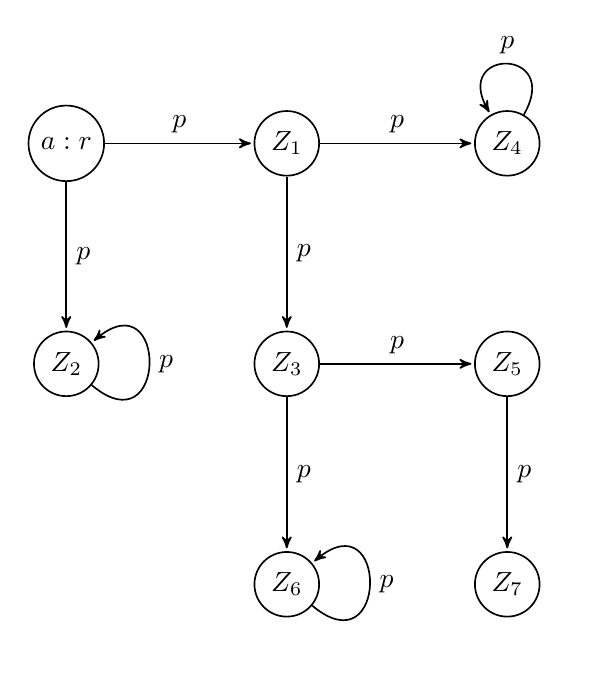
\begin{tikzpicture}[->,>=stealth',shorten >=1pt,auto,node distance=2.8cm,semithick]
  \tikzstyle{every state}=[circle,text=black,minimum size=0.1cm]

  \node[state] 						(A)              {$a:r$};
  \node[state]      			   	(B) [right of=A] {$Z_1$};
  \node[state]         				(C) [right of=B] {$Z_4$};
  \node[state]			    		(D) [below of=A] {$Z_2$};
  \node[state]			    		(E) [below of=B] {$Z_3$};
  \node[state]			    		(F) [below of=C] {$Z_5$};
  \node[state]			    		(G) [below of=E] {$Z_6$};
  \node[state]			    		(H) [below of=F] {$Z_7$};

  \path (A) edge              					node 		{$p$} 	(B)
            edge              					node 		{$p$} 	(D)
        (B) edge 			 					node 		{$p$} 	(E)
            edge              					node 		{$p$} 	(C)
        (C) edge [out=60,in=120,looseness=6]    node[above] {$p$} 	(C)
        (D) edge [out=320,in=40,looseness=6]	node[right] {$p$} 	(D)
        
        (E) edge 								node 		{$p$} 	(F)
        	edge 			 					node 		{$p$} 	(G)
        (F) edge 								node 		{$p$} 	(H)
        (G) edge [out=320,in=40,looseness=6]	node[right] {$p$} 	(G);
\end{tikzpicture}
\label{fig:ex_local_core}
\end{figure}

\begin{figure}[H]
    \centering
    \caption{Core chase}
    \vspace{11pt}
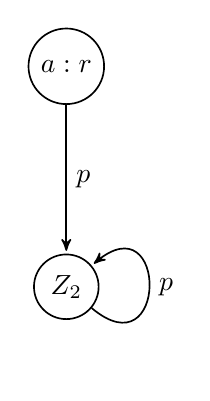
\begin{tikzpicture}[->,>=stealth',shorten >=1pt,auto,node distance=2.8cm,semithick]
  \tikzstyle{every state}=[circle,text=black,minimum size=0.1cm]

  \node[state] 						(A)              {$a:r$};
  \node[state]			    		(D) [below of=A] {$Z_2$};

  \path (A) edge              					node 		{$p$} 	(D)

        (D) edge [out=320,in=40,looseness=6]	node[right] {$p$} 	(D);
\end{tikzpicture}
\label{fig:ex_core}
\end{figure}

$h= \{(a,a),(z_2,z_2),(z_1,z_2),(z_3,z_2) \}$

\begin{center}
\begin{tabular}{|c|c|}
    \hline
    $\mathcal{F}$ & Atomes \\ 
    \hline
    1 & $\mathcal{F} \cup \{p(a, z_1)\} $\\
    \hline
    2 & $\{r(a),p(a, z_2),p(z_2, z_2)\} $\\
    \hline
    %\mathcal{F}_2 = \mathcal{F}_1 \cup \{p(a, z_2)\} & \mathcal{F}_2 = \mathcal{F}_1 & &\\
    %\hline
    %\mathcal{F}_{i+1} = \mathcal{F}_i \cup \{p(a, z_{i+1})\} &  & & \\
     %\hline
\end{tabular}
\end{center}



\end{example}
%%%%%%%%%%%%%%%%%%COMMENTE%%%%%%%%%%%%%%%%%%%%%%%%%%%%%%%%%%%%%%
\begin{comment}
\begin{tikzpicture}[->,>=stealth,shorten >=1pt,auto,node distance=4cm,
                thick,main node/.style={circle,draw,font=\Large\bfseries}]
  \node[main node] (1) {$a$};
  \node[main node] (2) [below left of=1] {$Z_0$};
  \node[main node] (3) [below right of=1] {$Z_1$};
  \node[main node] (4) [below of=2] {$Z_2$};

  \path
    (1) edge [loop above] node {r} (1)
        edge node {p} (3)
        edge node {p} (2)
    (2) edge node {p} (4)
    (3) edge [loop right] node {p} (3)
\end{tikzpicture}
\end{comment}
%%%%%%%%%%%%%%%%%%%%%%%%%%%%%%%%%%%%%%%%%%%%%%%%%%%%%%%
\newpage
\section{Conception et implémentation}\label{sec:conception_implementation}
    \subsection{Conception et implémentation des chases}
        \subsubsection{Analyse de l'existant dans Graal}
        \begin{figure}[H]
        \centering
        \includegraphics[width=\textwidth]{pictures/DiagrammeClasse.png}
        \caption{Diagramme de classes GRAAL}
        \label{fig:dclasse}
        \end{figure}
        
        Dans cette partie nous analysons ce qui était déjà présent sur GRAAL pour les \textit{chases}.
        
        Le package graal-forward-chaining est compris par 3 packages :
        \begin{itemize}
            \item \textit{Chase} : Il contient les implémentations des différentes \textit{chases} ( BreadthFirst, GRD, etc )
            \item \textit{HaltingCondition} : Une halting condition sert à tester si un trigger (R,h) est "actif" et s'il l'est la règle est appliquée par rapport à h.
            \item \textit{RuleApplier} : Un rule applier sert à calculer tous les homomorphismes du Body d'une règle dans F et ensuite il utilise les homomorphismes trouvés pour appliquer la règle en utilisant une \textit{HaltingCondition}.
        \end{itemize}
        
        \paragraph{Package Chase}\ \\
        Le package \textit{Chase} est compris d'une interface \textit{IChase} étant implementé par tous les \textit{chases} dans GRAAL. D'une classe abstraite AbstractChase qui implemente des versions génériques pour les méthodes de \textit{chases}. Enfin on a les différentes classes implementant different type de \textit{chases}.\\
        Le \textit{BasicChase} est une implémentation basique du \textit{chases} en largeur sans aucune optimisation. \\
        Le \textit{BreadthFirstChase} est une implémentation optimisée du \textit{chase} en largeur. Une première optimisation est l'utilisation de \textit{nouvFaits} à la fin de chaque étape pour déterminer quelles règles seront déclenchées à l'étape prochaine. On détermine aussi parmi ces règles lesquelles sont linéaires (avec un seul atome dans le body) pour stocker les atomes à utiliser pour le calcul des homomorphismes de façon à ce que ce dernier prenne en entrée une petite collection d'atomes plutôt que la base la base de faits entière. \\
        Le \textit{ChaseWithGRD} est un \textit{chase} qui utilise le graphe de dépendance des règles.\\
        Le \textit{SccChase} est un \textit{Chase} qui sature chaque composante fortement connexe du graphe de dépendance des règles individuellement. on l'utilise par la classe statique \textit{StaticChase}.\\
        Enfin le \textit{ChaseWithGRDAndUnfiers} est un \textit{chase} utilisant le graphe de dépendance des règles et des unificateurs.
        
        %\begin{itemize}
            %\item IChase : Interface qui doit être implémenté par tous les chases dans GRAAL.
            %\item AbstractChase : Classe abstraite qui implémente des versions génériques pour les méthodes des chases.
            %\item BasicChase : Implémentation basique du chase en largeur sans aucune optimisation.
            %\item BreadthFirstChase : Implémentation optimisée du chase en largeur. Une première optimisation est l'utilisation de nouvFaits à la fin de chaque étape pour déterminer quelles règles seront déclenchées à l'étape prochaine. On détermine aussi parmi ces règles lesquelles sont linéaires (avec un seul atome dans le body) pour stocker les atomes à utiliser pour le calcul des homomorphismes de façon à ce que ce dernier prenne en entrée une petite collection d'atomes plutôt que la base la base de faits entière.
            %\item ChaseWithGRD : Chase qui utilise le graphe de dépendance des règles.
            %\item SccChase : Chase qui sature chaque composante fortement connexe du graphe de dépendance des règles individuellement.
            %\item StaticChase : Classe statique qui permet d'utiliser le SccChase.
            %\item ChaseWithGRDAndUnfiers : Chase utilisant le graphe de dépendance des règles et des unificateurs.
        %\end{itemize}
        
        \paragraph{Package Halting Condition}\ \\
        Le package Halting Condition permet normalement de définir les différentes conditions d'arrêt pour la saturation des \textit{chases}. Mais ici un Halting condition teste plutôt si un trigger est actif avant de l'appliqué le cas échéant.\\ 
        Il est composé de l'interface IChaseHaltingCondition qui est implémenté par toutes les halting conditions. On ainsi deux classes:\\
        La FrontierRestrictedChaseHaltingCondition est utilisée par le semi-oblivious chase. \\
        La RestrictedChaseHaltingCondition est utilisée par le restricted chase.
        %\begin{itemize}
            %\item IChaseHaltingCondition : Interface à implémenter pour toutes les halting conditions. 
            %\item FrontierRestrictedChaseHaltingCondition : HaltingCondition utilisée par le semi-oblivious chase.
            %\item RestrictedChaseHaltingCondition : HaltingCondition utilisée par le restricted chase.
        %\end{itemize}

        \paragraph{Package RuleApplier}\ \\
        Le package RuleApplier est le package qui définit comment se s'applique les règles lors d'un \textit{chase}. Il est composé de l'interface IRuleApplier qui est implementée par tous les rules appliers. Nous avons ici 4 classes de rule applier:\\
        Le DefaultRuleApplier calcule tous les homomorphismes puis ne garde que la frontière de chacun.\\
        L'ExhaustiveRuleApplier calcule tous les homomorphismes et les garde sans aucune modification.\\
        Le RestrictedChaseRuleApplier est spécifiquement optimisé pour le restricted chase.\\
        Le DefaultRuleApplierWithCompilation est un Rule Applier qui utilise des règles avec compilation.
        
        %\begin{itemize}
            %\item IRuleApplier : Interface à implémenter pour tous les rules appliers. 
            %\item DefaultRuleApplier : Il calcule tous les homomorphismes puis ne garde que la frontière de chacun.  
            %\item ExhaustiveRuleApplier : Il calcule tous les homomorphismes et les garde sans aucune modification.
            %\item RestrictedChaseRuleApplier : Rule Applier spécifiquement optimisé pour le restricted chase. 
            %\item DefaultRuleApplierWithCompilation : Rule Applier qui utilise des règles avec compilation.
        %\end{itemize}
        
        \begin{figure}[H]
        \centering
        \includegraphics[width=\textwidth]{pictures/DiagrammeSequence.png}
        \caption{Diagramme de sequence next()}
        \label{fig:dsequence}
        \end{figure}
        
        Pour que le diagramme de sequence et donc le fonctionnement des chases soit plus comprehensible il nous semblait important de revenir sur la fonction \textit{next()} et sur son fonctionnement.
        
        \paragraph{Fonction \textit{next()}}\ \\
        La fonction next() fait une étape de largeur de l'algorithme chase en parallèle. Cette fonction utilise deux hashmaps du type Map<Rule, AtomSet> pour stocker les règles qui devront être appliquées à l'étape suivante et les atomes qui seront utilisés pour le calcul des homomorphismes, ces deux hashmaps s'appellent rulesToCheck et nextRulesToCheck. Avant le premier appel à la méthode on initialise nextRulesToCheck avec toutes les règles de la base de règles de la façon suivante : $nextRulesToCheck({R}) = <{R},\mathcal{F}> $. À chaque appel de la méthode next on suit les étapes suivantes : 
        \\
        
        \begin{itemize}
        \item On copie $nextRulesToCheck$ dans $rulesToCheck$, et on réinitialise $nextRulesToCheck$.
        \item Pour chaque règle $R_i$ dans $rulesToCheck$ on appelle la fonction $delegatedApply$ dans RuleApplier qui va calculer tous les homomorphismes du corps de la règle vers la base de faits de l'étape précédente, puis, pour chacun de ces homomorphismes on appelle la fonction $apply$ dans HaltingCondition et on génère les atomes s'ils ne sont pas redondants par rapport au critère choisi, c'est-à-dire, on applique l'homomorphisme à la tête de la règle.
        \item Les atomes génerés par HaltingCondition sont renvoyés au BreadthFirstChase à travers RuleApplier. Ces atomes sont stockés par BreadthFirstChase dans nouvFaits puis on continue avec la règle suivante.
        \item Quand on a traité toutes les règles on appelle $dispatchNewData$ qui va prendre tous les nouveaux atomes générés, et pour chacun de ces atomes cette fonction teste sur chacune des règles de $\mathcal{BR}$ si cet atome $\alpha$ apparaît dans le corps de la règle. 
        \item S'il n'appartient pas au corps de la règle on continue avec la règle suivante, mais s'il appartient on a deux cas; soit la règle n'est pas linéaire alors on l'ajoute dans $nextRulesToCheck(R_i,\mathcal{BF})$, soit elle est linéaire et n'a pas déjà été ajoutée dans $nextRulesToCheck$ dans ce cas on l'ajoute dans $nextRulesToCheck(R_i, \alpha)$. Sinon on ajoute l'atome $\alpha$ dans la liste associé à la règle dans $nextRulesToCheck(R_i)$. 
        \end{itemize}
        
        \paragraph{Critique}
        Face à cette organisation et dans l'idée de proposer notre propre itération d'une implémentation des chases  nous avons donc était amené à nous demandé qu'elles étaient les choses pouvant être améliorées.\\
        Tout d'abord le nom du package HaltingCondition n'est pas le plus clair, une halting condition devrait normalement être une condition d'arrêt pour la saturation d'un chase, mais ici, elles testent si un trigger est actif et ensuite l'appliquent.\\
        Ensuite nous avons remarqué que l'implémentation génériques des chases n'utilisé pas les notions d'extensions locale et d'extensions globale, GRAAL fait toujours l'union ce qui pourrait être amélioré.\\
        Nous avons aussi remarqué qu'il existe des classes qui ne sont pas utiles ou pas encore finies. StaticChase ou HaltingConditionWithHandler en sont des exemples.\\
        Enfin nous nous sommes rendus compte que dans l'implémentation actuelle de Graal, les homomorphismes sont recalculés intégralement à chaque étape du chase, ce qui ralentit considérablement le calcul de la base de faits saturée.
        %\begin{itemize}
            %\item Nous ne trouvons pas que le package HaltingCondition est bien nommé, une halting condition devrait normalement être une condition d'arrêt pour la saturation d'un chase, mais ici, elles testent si un trigger est actif et ensuite l'appliquent.
            %\item Pour avoir des implémentions vraiment génériques des chases il faudrait rajouter les notions d'extension locale et d'extension globale, Graal fait toujours l'union.
            %\item Il existe des classes qui ne sont pas utiles ou pas encore finies. StaticChase ou HaltingConditionWithHandler en sont des exemples. 
            %\item Dans l'implémentation actuelle de Graal, les homomorphismes sont recalculés intégralement à chaque étape du chase, ce qui ralentit considérablement le calcul de la base de faits saturée.
        %\end{itemize}
        
        %\subsubsection{Conception}
     %\subsection{Conception et implémentation des simplificateurs de bases de règles}
     
     
    \subsubsection{Analyse du nouveau travail dans Graal}
        \begin{figure}[H]
        \centering
        \includegraphics[width=\textwidth]{pictures/NouveauDiagrammeClasse.png}
        \caption{Nouveau Diagramme de classes GRAAL // needs updating}
        \label{fig:dclasse}
        \end{figure}
        
    Dans cette partie nous développerons le travail que nous avons fait sur l'implémentation des \textit{chases} que nous proposons. L'organisation des classes, les fonctions utilisées et de manière générale les problèmes que nous avons rencontré et au final comment cette nouvelle version est sensée fonctionner.
    
    \paragraph{Package Chase}\ \\
    Pour l'implémentation des \textit{chases} nous avons mis en place une interface Chase reprenant les fonctions \textit{execute()} et \textit{execute(HaltingCondition)} servant à exécuter l'algorithme \textit{chase} en ajoutant un condition d'arrêt.
    Cette interface est héritée par la classe abstraite \textit{AbstractChase} qui implémente les versions générique des \textit{chases}. On a aussi l'interface \textit{BreadthFirstChase} (resp. \textit{BreadthFirstChase}) qui représente l'interface qui doit être implémentée par les \textit{chases} en largeur (resp.profondeur).
    Enfin on a la classe \textit{classicBreadthFirstChase} fonctionnant pour les exécutions en largeur et la classe \textit{ParralelBreadthFirstChase} fonctionnant pour les exécutions en parallèle. On a fait la différence entre les deux parce que la version en parallèle n’est pas affecté par l’ordre d’application de règles alors qu'une version en largeur est sensible à l’ordre d’application de règles.
        %\begin{itemize}
            %\item Chase : Interface qui doit être implémentée par tous les chases dans GRAAL.
            %\item AbstractChase : Classe abstraite qui implémente des versions génériques pour les méthodes des chases.
            %\item DepthFirstChase : Interface qui doit être implémentée par tous les chases en profondeur.
            %\item BreadthFirstChase : Interface qui doit être implémentée par tous les chases en largeur.
            %\item AbstractBreadthFirstChase : Classe abstraite qui implémente des versions génériques pour les méthodes des chases en largeur.
            %\item ParallelBreadthFirstChase : Classe qui implémente les chases en parallèle.
            %\item NotParallelBreadthFirstChase : Classe qui implémente les chases en largeur.
        %\end{itemize}
        
    \paragraph{Package Trigger Checker}\ \\
    Pour le test d'applicabilité des règles nous avons mis en place une interface \textit{TriggerChecker} reprenant la fonction \textit{check} qui nous répond par vrai si une règle donnée est applicable pour un homomorphisme et la base de faits données et faux sinon. Et nous avons différentes classes pour les différents implémentations pour le test d'applicabilité. La classe qui vérifie l'applicabilité de l'Oblivious chase par la méthode check et donc va retourner toujours vrai. Voir l'algorithme \ref{algo:est_applicable_oblivious}. La classe qui étend l'ObliviousTriggerChecker en vérifiant l'applicabilité du SemiOblivious chase par la méthode check. Voir l'algorithme \ref{algo:est_applicable_semi_oblivious}. Et finallement la classe qui étend le SemiObliviousTriggerChecker en  vérifiant l'applicabilité du Restricted chase par la méthode check. Voir l'algorithme \ref{algo:est_applicable_restricted}.
        \\
        %\begin{itemize}
            %\item TriggerChecker : Interface qui doit être implémenté par tous les TriggerChecker dans GRAAL.
            %\item ObliviousTriggerChecker : Classe qui vérifie l'applicabilité de l'Oblivious chase par la méthode check. Voir l'algorithme \ref{algo:est_applicable_oblivious}. % retourne toujours vrai
            %\item SemiObliviousTriggerChecker : Classe qui étend l'ObliviousTriggerChecker en  vérifiant l'applicabilité du SemiOblivious chase par la méthode check. Voir l'algorithme \ref{algo:est_applicable_semi_oblivious}.
            %\item RestrictedTriggerChecker : Classe qui étend le SemiObliviousTriggerChecker en  vérifiant l'applicabilité du Restricted chase par la méthode check. Voir l'algorithme \ref{algo:est_applicable_restricted}.
        %\end{itemize}
        
    \paragraph{Package Halting Condition}\ \\
    Pour éviter les cas où l'exécution d'un \textit{chase} ne termine pas, nous avons dû ajouter un condition d'arrêt. On a mis en place une interface \textit{HaltingCondition} (resp. \textit{BFCHaltingCondition}) reprenant la fonction \textit{isFinished} qui nous dit si l'exécution des \textit{chases} (resp. en largeur) est terminée ou non. \textit{HaltingCondition} (resp. \textit{BFCHaltingCondition}) est héritée par la classe abstraite \textit{AbstractHaltingCondition} (resp. \textit{AbstractBFCHaltingCondition}) qui implémente les conditions d'arrêt pour les différents \textit{chases} (resp. \textit{chases} en largeur). On a deux conditions d'arrêt la première consiste à tester si l'exécution a dépassé un certain nombre d'étapes c'est pourquoi on a la classe \textit{LimitStepsHaltingCondition} et la seconde avec la classe \textit{TimeoutHaltingCondition} consiste à tester si l'exécution a dépassé un certain temps donné.
        %\begin{itemize}
            %\item HaltingCondition : Interface qui doit être implémentée pour définir les différentes conditions d'arrêt dans GRAAL.
            %\item BFCHaltingCondition : Interface qui doit être implémenté pour définir les conditions d'arrêt des chases en largeur dans GRAAL.
            %\item LimitStepsHaltingCondition : Classe qui implémente la condition d'arrêt par nombres d'étapes.
            %\item AbstractHaltingCondition : Classe abstraite qui implémente les conditions d'arrêt pour les différents chases.
            %\item AbstractBFCHaltingCondition : Classe abstraite qui implémente les conditions d'arrêt pour les différents chases en largeur.
            %\item TimeoutHaltingCondition : Classe qui implémente la condition d'arrêt par rapport au temps d'exécution.
        %\end{itemize}
        
        
    \paragraph{Package Rule Applier}\ \\
    Après le test d'applicabilité, si une règle est applicable il faut l'appliquer. Pour l'application des règles on a mis en place une interface \textit{BreadthFirstRuleApplier} qui implemente une classe abstraite \textit{AbstractBreadthFirstRuleApplier} qui sert pour l'implementation des \textit{chases} en largeur, ainsi que deux classes \textit{DefaultBreadthFirstRuleApplier} et \textit{RestrictedBreadthFirstRuleApplier} qui reprenent la fonction \textit{applyRule}. Cette dernière applique la règle déjà validée par le \textit{Trigger Checker}.     
        %\begin{itemize}
            %\item BreadthFirstRuleApplier : Interface qui doit être implémentée pour l’application des règles pour les méthodes des chases en largeur dans GRAAL
            %\item AbstractBreadthFirstRuleApplier : Classe abstraite qui implémente l'application des règles pour les méthodes des chases en largeur.
            %\item DefaultBreadthFirstRuleApplier : Classe qui implémente l'application des règles avec la fonction \textit{applyRule}.
            %\item RestrictedBreadthFirstRuleApplier : Classe qui implémente l'application des règles avec la fonction \textit{applyRule}.
        %\end{itemize}
        
        
    \paragraph{Package Extender} 
    Le package \textit{Extender} reprend les classes qui permettent d'étendre la base de faits lors des processus de chase grace aux nouveaux homomorphismes. Il est composé de deux interfaces l'une pour l'extension locale, \textit{LocalAtomsSetExtender}, l'autre pour une extension au niveau global, \textit{GlobalAtomSetExtender}, ainsi que d'une classe abstraite, \textit{AbstractExtender}, qui implemente des version générique de la méthode \textit{extend()}($extend():$ est la méthode qui reprend les algos\ref{algo:etendre_general}, \ref{algo:etendre_local_defaut} et \ref{algo:etendre_chase} qui choisit lequel appliquer et l'applique.).\\
    On retrouve 5 classe:\\
    Le \textit{DefaultAtomSetExtender} qui gere l'extension pour les algo 'classique', Oblivious, semi-Oblivious, Restricted \textit{chases}.
    Puis 4 classes qui gere les extension locale et globale pour le \textit{CoreChase}, \textit{CoreAtomSetExtender}, pour le \textit{LocalCoreChase}, \textit{LocalAtomSetExtender}, puis pour le \textit{LocalVacuumChase}, \textit{VacuumLocalAtomSetExtender}, et le \textit{VacuumChase} avec le \textit{VacuumGlobalAtomSetExtender}. 
        %\begin{itemize}
            %\item LocalAtomSetExtender : Interface qui doit être implémentée par tous les LocalAtomSetExtender dans GRAAL.
            %\item GlobalAtomSetExtender : Interface qui doit être implémentée par tous les GlobalAtomSetExtender dans GRAAL.
            %\item AbstractExtender : Classe abstraite qui implémente des versions génériques de la méthode $extend()$.
            %\item DefaultAtomSetExtender : Classe qui applique le $extend()$ pour étendre la bases des faits.
            %\item CoreAtomSetExtender : Classe qui applique le $extend()$ pour le CoreChase.
            %\item LocalAtomSetExtender : Classe qui applique le $extend()$ pour le LocalCoreChase.
            %\item VacuumLocalAtomSetExtender : Classe qui applique le $extend()$ pour le LocalVacuumChase.
            %\item VacuumGlobalAtomSetExtender : Classe qui applique le $extend()$ pour le VacuumChase.
        %\end{itemize}
        
        %$extend():$ est la méthode qui reprend les algos\ref{algo:etendre_general}, \ref{algo:etendre_local_defaut} et \ref{algo:etendre_chase} qui choisit lequel appliquer et l'applique.
        
        
    \paragraph{Package Exception}
        \begin{itemize}
            \item RuleApplierException :
            \item AtomSetExtenderException :
            \item ChaseException :
            \item TriggerCheckerException :
        \end{itemize}
        
\newpage
\section{Expérimentation des chaînages avant}\label{sec:experimentation}
% les differentes experimentations faites pour comparer les differents chases
% commentaires pour chacun

Dans cette section nous présentons une évaluation exhaustive des différents \textit{chases}. Nous avons trois objectifs principaux en réalisant cette évaluation :

\begin{enumerate}
  \item Vérifier la correction des nos \textit{chases}.
  \item Comparer nos \textit{chases} à ceux qui existaient déjà dans Graal.
  \item Comparer tous les différents \textit{chases} implémentés. 
\end{enumerate}

\subsection{Méthode d'expérimentation}

Nous avons implémenté un outil de benchmarking qui nous permet de lancer tous les \textit{chases} (ceux que nous avons implémenté ainsi que ceux déjà existants dans Graal) avec des limites sur les temps globaux d'exécution, le temps d'exécution de chaque étape de largeur et le nombre des faits générés. Étant donné que les \textit{chases} peuvent facilement exploser en termes de temps d'exécution et de faits générés on a implémenté des limitations pour éviter d'obtenir des temps d'exécution trop longs et des possibles erreurs de mémoire. 

Le benchmark prends en entrée un fichier "dlp" avec la base des connaissances et lance chacun des \textit{chases} jusqu'à ce que la saturation se termine ou jusqu'à ce que l'une des trois conditions d'arrêt mentionnés précédemment soit atteinte. Une fois ce processus fini on sauvegarde comme résultat le temps d'exécution de chaque étape et le nombre de faits appartenant à la base de faits à la fin de chaque étape. Cela nous permets de faire des comparaisons détaillés entre tous les \textit{chases} exécutés.

%procède à la saturer itérativement avec chacun des chases jusqu'à ce que la saturation soit fini ou l'une des trois conditions d'arrêt mentionnés précédemment soit atteint.

Le nombre de faits générés nous permets de vérifier la correction de nos \textit{chases} par rapport a ceux existants dans Graal, une fois les \textit{chases} ont été corrigés le temps d'exécution nous permets de comparer l'efficacité de nos \textit{chases} par rapport à ceux déjà existants. Et finalement avec ces deux mesures nous pouvons aussi comparer tous les \textit{chases} en terme de vitesse d'exécution et de capacité à éviter des redondances.

\subsection{Bases de connaissances d'expérimentation}

Nous avons pris plusieurs bases de connaissances faites à la main pour tester les \textit{chases}, ces bases ont la particularité d'avoir peu de règles et peu des faits au départ tout en générant de nombreuses redondances. Cela nous permet de tester les limites des algorithmes après peu d'itérations. Nous avions aussi prévu d'exécuter des tests avec des bases de connaissances crées par la communauté scientifique dans le but explicite de pousser les algorithmes de \textit{chase} vers leurs limites. Malheureusement nous avons pas eu le temps de réaliser ces tests pendant le déroulement de ce TER, bien que certains de nos résultats soient intéressants, notre méthode de benchmark est assez naïve. Une batterie de tests plus soutenue sera donc à mettre en oeuvre pour améliorer la précision et la pertinence de nos résultats. Nos bases des connaissances d'expérimentation sont les suivants : 

\vspace{10pt}
\textbf{$\mathcal{KB}_A$}\\
$\mathcal{F} = \{p(a,b)\}$ \\
$R = p(X,Y) \rightarrow p(Y,Z), p(Z,Z), p(Z,X), p(X,U), p(U,Y), p(U,U)$\\

\textbf{$\mathcal{KB}_B$}\\
$\mathcal{F} = \{p(a,b)\}$ \\
$R = p(X,Y) \rightarrow p(Y,Z), p(Z,U), p(U,X), p(X,O), p(O,Q), p(Q,Y), p(U,U), p(Q,Q), p(O,O), p(Z,Z)$\\

\textbf{$\mathcal{KB}_C$}\\
$\mathcal{F} = \{p(c,d), p(a,b), p(e,f)\}$ \\
$R = p(X,Y), p(U,W) \rightarrow q(X,Z), q(Z,X), p(Z,V), q(U,Z), q(Z,U)$\\

\textbf{$\mathcal{KB}_D$}\\
$\mathcal{F} = \{p1(a), p1(n),q(b,f),q(f,c),q(b7,f5),q(f5,c5),q(b6,f6),q(f8,c8)\}$ \\
$R = p1(X), q(V,Y) \rightarrow p1(Z),p(X,Z),q(V,Z)$\\

\textbf{$\mathcal{KB}_E$}\\
$\mathcal{F} = \{b(a), c(a)\}$\\
$R1 = b(X) \rightarrow p(X,Z)$\\
$R2 = p(X,Y) \rightarrow p(X,Z), a(Z)$\\
$R3 = p(X,Y), a(W) \rightarrow p(Y,Z)$\\
$R4 = p(X,Y), a(Y) \rightarrow p(Y,Y)$\\
$R5 = p(X,Y), c(X) \rightarrow q(Y)$\\

\textbf{$\mathcal{KB}_F$}\\
$\mathcal{F} = \{p(a,b), p(b,c), p(c,d)\}$\\
$R = p(X,Y) \rightarrow p(Y,Z), p(Z,Z), p(Z,X), p(X,U), p(U,Y), p(U,V), p(V,Z), p(V,V), p(X,A), p(A,B), p(B,Y)$

\subsection{Résultats}

Toutes les expérimentations ont été réalisés sur un seul ordinateur avec un processeur AMD FX-8350 et 16Go de mémoire. Les paramètres d'arrêt utilisés lors du benchmark sont 1 heure de temps de exécution globale, 30 minutes maximum par étape et 1.000.000 de faits générés.

\subsubsection{Comparaison Graal Chases et Nouveaux Chases}
Nous commençons pour vérifier la correction de nos algorithmes, pour ce faire nous avons lancé le benchmark pour les 6 bases de connaissances mentionnés précédemment et nous comparons le nombre de faits générés à la dernière étape par tous les algorithmes. Les résultats sont présentés dans le tableau \ref{tab:faitsoldnew}.


\begin{table}[H]
\begin{center}
\begin{tabular}{|c|c|c|c|c|} 
    \hline
    $\mathcal{KB}$/Étape & \shortstack{New \\ Semi-oblivious Chase}  & \shortstack{Graal \\ Semi-oblivious Chase} & \shortstack{New \\ Parallel Restricted Chase} & \shortstack{Graal \\ Parallel Restricted Chase} \\
    \hline
     \hline
    $\mathcal{KB}_A$/6 & 55987 & 55987 & 1375 & 1375 \\ 
     \hline
    $\mathcal{KB}_B$/5 & 111111 & 111111 & 3851 & 3851 \\ 
    \hline
    $\mathcal{KB}_C$/4 & 107754 & 107754 & 21882 & 21882 \\ 
    \hline
    $\mathcal{KB}_D$/4 & 1556 & 1556 & 1556 & 152324 \\ 
    \hline
    $\mathcal{KB}_E$/13 & 754 & 754 & 332 & 332 \\ 
     \hline
    $\mathcal{KB}_F$/4 & 48315 & 48315 & 24918 & 24918 \\ 
     \hline 
\end{tabular}    
\caption {Comparaison \textit{Graal Chases} - \textit{Nouveaux Chases}} \label{tab:faitsoldnew}
\end{center}
\end{table}

Les résultats sont correct, en effet, nous pouvons constater que le \textit{graal semi-oblivious chase} et le \textit{nouveau semi-oblivious chase} génèrent la même quantité d'atomes, le \textit{graal restricted chase} et le \textit{nouveau restricted chase} génerènt aussi la même quantité d'atomes sauf dans le cas du $\mathcal{KB}_D$ où le \textit{graal restricted chase} génère même plus d'atomes que le \textit{graal semi-oblivious chase}. Cela s'explique car il y a un bug dans la classe BacktrackHomomorphism de Graal.

Maintenant que nous avons validé la correction de nos \textit{chases}, nous allons comparer les temps d'exécution du \textit{semi-oblivious chase} et \textit{restricted chase} qui sont implémentés dans Graal avec nos nouvelles versions. Les graphiques présentées ci-dessous montrent le temps en millisecondes (axe Y) en fonction de l'étape de largeur (axe X). L'axe temps a été mis en échelle avec une fonction logarithme pour que les graphes restent lisibles. Les tableaux utilisés pour construire tous ces graphiques se trouvent dans l'annexe B.

Prenons les résultats de $\mathcal{KB}_A$ (Fig. \ref{fig:ex0oldnew}), nous pouvons voir que dans le cas du \textit{semi-oblivious chase} la nouvelle implémentation est plus lente que celle de Graal lors des premières étapes quand la base des faits est petite, après quand la base de faits commence à grandir la nouvelle implementation deviens considérablement plus rapide. On remarque que l'implementation de Graal fait un timeout pendant le calcul de l'étape 7, ce qui explique que la courbe fini à l'étape 6, alors que la nouvelle implémentation arrive à calculer deux étapes de plus. Nous observons des résultats similaires avec le \textit{restricted chase}, c'est un peu difficile à constater dans le graphique due à l'échelle logarithmique utilisé mais le \textit{nouvel restricted chase} a réalisé 12 étapes de largeur en 23 minutes tandis que la version de Graal a mis 25 minutes et demi pour faire le même calcul. Cette amélioration en temps de calcul est due principalement à notre méthode de calcul des nouveaux homomorphismes qui nous évite de faire des calculs redondants tandis-que que l'implémentation de Graal calcule tous les homomorphismes à chaque étape de largeur.

\begin{figure}
\centering
\includegraphics[width=\textwidth]{pictures/benchmark_old-new/ex0oldnew.png}
\caption{$\mathcal{KB}_A$ }
\label{fig:ex0oldnew}
\end{figure}

\begin{figure}
\centering
\includegraphics[width=\textwidth]{pictures/benchmark_old-new/ex1oldnew.png}
\caption{$\mathcal{KB}_B$}
\label{fig:ex1oldnew}
\end{figure}

\begin{figure}
\centering
\includegraphics[width=\textwidth]{pictures/benchmark_old-new/ex2oldnew.png}
\caption{$\mathcal{KB}_C$}
\label{fig:ex2oldnew}
\end{figure}

\begin{figure}
\centering
\includegraphics[width=\textwidth]{pictures/benchmark_old-new/ex11oldnew.png}
\caption{$\mathcal{KB}_D$}
\label{fig:ex11oldnew}
\end{figure}

\begin{figure}
\centering
\includegraphics[width=\textwidth]{pictures/benchmark_old-new/exampleoldnew.png}
\caption{$\mathcal{KB}_E$}
\label{fig:exampleoldnew}
\end{figure}

\begin{figure}
\centering
\includegraphics[width=\textwidth]{pictures/benchmark_old-new/moldnew.png}
\caption{$\mathcal{KB}_F$}
\label{fig:moldnew}
\end{figure}

Nous observons des résultats similaires dans les autres exemples, avec deux exceptions à noter, premièrement, dans $\mathcal{KB}_B$ (Fig. \ref{fig:ex1oldnew}) le \textit{nouvel restricted chase} prends 27 secondes de plus pour calculer 12 étapes que le \textit{restricted chase} de Graal, cela peut s'expliquer dpar le fait que l'on a pris qu'une seule mesure, en refaisant l'expérimentation ou en la laissant tourner une étape de plus on devrait atteindre de meilleurs résultats. Deuxièmement, dans $\mathcal{KB}_D$ le temps de calcul du \textit{restricted chase} de Graal augmente de façon exponentielle due au bug trouvé dans la classe BacktrackHomomorphism de Graal.

Après avoir réalisés ces expérimentations nous pouvons conclure que notre implémentation des \textit{chases} montrent des résultats satisfaisants qui se démarque au fur et au mesure que la base de faits qu'on est en train de saturer grandis. 

\subsubsection{Comparaison Nouveaux Chases}

Maintenant nous allons comparer tous les chases que nous avons implementé, c'est-à-dire, les nouvelles versions du \textit{restricted chase}, le \textit{core chase}, le \textit{local core chase} et le \textit{vacuum chase}. La méthode employé ici est la même que précédemment mais nous cherchons plutôt ici à comparer les différents types de \textit{chase}.

Avec la base de connaissances $\mathcal{KB}_A$ (Fig. \ref{fig:ex0newfacts} et  Fig. \ref{fig:ex0newtime}) nous observons que le \textit{local core chase} et le \textit{core chase} finissent la saturation lors de l'étape 4 avec 31 faits générés, la différence de temps entre les deux n'est pas significative dans cette exemple. Le \textit{vacuum chase} et le \textit{parallel restricted chase} montrent des résultats similaires jusqu'à l'étape 6, lors de l'étape 7 le \textit{vacuum chase} semble même être meilleur pendant un temps avant de se mettre à générer plus des redondances que le \textit{restricted chase}. Cette irrégularité semble indiqué un problème avec notre implémentation du \textit{vacuum chase}. 

\begin{figure}
\centering
\includegraphics[width=\textwidth]{pictures/benchmark_new/ex0newfacts.png}
\caption{$\mathcal{KB}_A$ Faits générés}
\label{fig:ex0newfacts}
\end{figure}

\begin{figure}
\centering
\includegraphics[width=\textwidth]{pictures/benchmark_new/ex0newtime.png}
\caption{$\mathcal{KB}_A$ Temps}
\label{fig:ex0newtime}
\end{figure}

Dans la base de connaissances $\mathcal{KB}_E$ (Fig. \ref{fig:examplenewfacts} et  Fig. \ref{fig:examplenewtime}) nous pouvons remarquer que l'algorithme qui prend le plus de temps c'est le \textit{parallel restricted chase}, cela est du au fait qu'il génère de nombreux faits redondants. Le \textit{vacuum chase}, lui, est capable d'éliminer un grand nombre des faits redondants ce qui le rends plus efficace que le \textit{parallel restricted chase} en temps d'exécution aussi qu'en quantité des faits générés. Le \textit{local core chase} et le \textit{breadth first restricted chase}, eux, sont équivalents en termes de faits produits, cela peut s'expliquer par le fait que le \textit{breadth first restricted chase} a un ordre d'application des règles qui est équivalent au \textit{local core chase}. Comme attendu le \textit{breadth first chase} est beacoup plus rapide que le \textit{local core chase} car il fait moins des calculs. Finalement, Le \textit{core chase}, fini ici en 5 étapes avec une base de faits contenant 6 faits ce qui fait de lui l'algorithme le plus efficace en nombre de faits produits. Il obtient aussi le meilleur temps car, contrairement aux autres algorithmes, il fini sa saturation.

\begin{figure}
\centering
\includegraphics[width=\textwidth]{pictures/benchmark_new/examplenewfacts.png}
\caption{$\mathcal{KB}_E$ Faits générés}
\label{fig:examplenewfacts}
\end{figure}

\begin{figure}
\centering
\includegraphics[width=\textwidth]{pictures/benchmark_new/examplenewtimes.png}
\caption{$\mathcal{KB}_E$ Temps}
\label{fig:examplenewtime}
\end{figure}

Puis, en utilisant $\mathcal{KB}_F$ (Fig. \ref{fig:mnewtime} et Fig. \ref{fig:mnewfacts}) nous observons que le \textit{core chase} arrive à enlever plus des redondances que le \textit{local core chase}, néanmoins ce dernier reste beaucoup plus rapide. Il prends 6 minutes et demi pour finir 3 étapes de largeur pendant que le \textit{core chase} à besoin d'environ 16 minutes. Il faut remarquer que les deux algorithmes font un timeout l'étape 4 leurs prenant plus de 30 minutes. Le \textit{vacuum chase} arrive à enlever des redondances que le \textit{parallel restricted chase} n'est pas capable de détecter, néanmoins il est considérablement plus lent. en fait il n'arrive à finir que 4 étapes de largeur avant d'atteindre le timeout tandis que le \textit{parallel restricted chase} a pu finir 5 étapes de largeur. 
%à besoin d'environ 16 minutes pour calculer 6 étapes ( faux il me semble que c'est 3 étapes a vérifier!)

\begin{figure}
\centering
\includegraphics[width=\textwidth]{pictures/benchmark_new/mnewtimes.png}
\caption{$\mathcal{KB}_F$ Temps}
\label{fig:mnewtime}
\end{figure}

\begin{figure}
\centering
\includegraphics[width=\textwidth]{pictures/benchmark_new/mnewfacts.png}
\caption{$\mathcal{KB}_F$ Faits générés}
\label{fig:mnewfacts}
\end{figure}

Nous pouvons observer que le \textit{local core chase} et le \textit{vacuum chase} se trouvent entre le \textit{restricted chase} et le \textit{core chase}, en termes de temps mais aussi en termes de redondances détectés. il faut aussi remarquer que de façon général le \textit{local core chase} élimine plus de redondances que le \textit{vacuum chase} mais il est aussi plus lent. Le calcul du core reste un calcul compliqué même quand la base de faits est pré-gelée. Dans les cas où le calcul du core permets l'arrêt de la saturation, le \textit{core chase} est l'algorithme le plus puissant.

\par Après avoir étudié la suppression des redondances dans le cadre du chaînage avant, on va présenter la suppression des redondances dans les règles.
\newpage
\section{Suppression des redondances dans les règles}\label{sec:regles}

\par Dans cette partie on va s'intéresser à un autre type de redondance : les redondances dans les bases de règles. Plus précisément, on s'est intéressé à deux formes particulières : 
%Une autre façon de supprimer des redondances est d'analyser la base de règles. Dans le cadre de ce projet nous avons étudié deux formes de redondances : 
\begin{itemize}
    \item les redondances au sein d'une seule et même règle, que l'on nommera redondances intra-règles (\ref{sec:intra-regles}) ;
    \item les redondances de règles par rapport aux autres règles, que l'on nommera redondances inter-règles (\ref{sec:inter-regles}).
\end{itemize}
Nous avons étudier ces redondances à l'aide de deux articles : \textit{Redundancy Rules Reduction in Rule-Based Knowledge Bases, Yongjie Zhang, Ansheng Deng} \cite{DBLP:conf/fskd/2015} et \textit{Theory and Algorithm for Rule Base Refinement, Hai Zhuge, Yunchuan Sun, Weiyu Guo} \cite{DBLP:conf/ieaaie/2003} ainsi qu'un document \cite{MINIREGLE} écrit pendant le stage d'un membre du groupe.
\par Puis on présentera une application s'appuyant sur Graal permettant de supprimer ces redondances (\ref{sec:conception-RAMIX}).


\subsection{Redondances intra-règles}\label{sec:intra-regles}
\par Avant d'entrer plus dans les détails on posera une règle de la forme $R = B \rightarrow H$ et on notera $R' = \linebreak frontierFreeze(R) =  (B' \rightarrow H')$ la règle $R$ où la frontière est gelée. 
\par On distingue deux formes de redondances intra-règles : les redondances au sein du corps de la règles (\ref{sec:redondances_corps}) et les redondances de la tête dans le corps et la tête de la règle (\ref{sec:redondances_tete_corps}).

\subsubsection{Redondances dans le corps de la règle}\label{sec:redondances_corps}
\par Il existe des redondances au sein du corps $B$ de la règle $R$ si et seulement si le nombre d'atomes dans le \textit{core} (\ref{def:Core}) de $B'$ est strictement inférieur au nombre d'atomes dans $B'$. 
\par Pour bien comprendre l'intérêt de supprimer ce type de redondance, on peut prendre l'exemple de la règle $R_1 = p(X) \land p(Y) \rightarrow q(X, Z)$. L'atome $p(Y)$ est redondant car il existe un homomorphisme : $h = \{ X \rightarrow X, Y \rightarrow X \} $ tel que $h(\{p(X), p(Y)\}) = \{p(X)\}$, donc il ne fait donc pas partie du \textit{core} de $B'$. La règle $R_1' = p(X) \rightarrow q(X, Z)$ est équivalente à $R_1$ et sans redondance dans le corps.
\par Comparons maintenant ces deux règles dans le cadre d'une saturation. Soit la base de faits $\mathcal{F} = \{p(a), p(b)\}$. Prenons tout d'abord la base de connaissance $\mathcal{KB}_1 = (\mathcal{F}, \{R_1\})$. Lors de la première étape de saturation, on peut trouver quatre déclencheurs : $(R_1,\{ X \rightarrow a, Y \rightarrow a\})$, $(R_1, \{ X \rightarrow a, Y \rightarrow b\})$, $(R_1, \{ X \rightarrow b, Y \rightarrow a\})$, $(R_1, \{ X \rightarrow b, Y \rightarrow b\})$. Si on sature à l'aide de l'\textit{oblivious chase} on obtiendrait la base de faits suivante $\mathcal{F}^*_A = \{p(a), p(b), q(a,Z_1), q(a,Z_2), q(b, Z_3), q(b, Z_4)\}$ dont le \textit{core} est $\{p(a), p(b), q(a,Z_1), q(b,Z_3)\}$. Si on prend maintenant la base de connaissance $\mathcal{KB}_2 = (\mathcal{F}, \{R_1'\})$, lors de la première étape de saturation, on peut trouver deux déclencheurs : $(R_1',\{ X \rightarrow a\})$, $(R_1', \{ X \rightarrow b\})$. Si on sature à l'aide de l'\textit{oblivious chase} on obtiendrait la base de faits suivantes $\mathcal{F}^{*}_B = \{p(a), p(b), q(a,Z_1), q(b,Z_2)\}$ qui est équivalente au \textit{core} de $\mathcal{F}^*_A$. 
\par Si on utilise les critères d'applicabilités du \textit{semi-oblivious chase} et du \textit{restricted chase}, ces redondances seraient évitées mais au prix d'un temps de calcul supplémentaire. D'où l'intérêt de supprimer ce type de redondance au sein des règles.


\paragraph{L'algorithme \textit{BodyRedundancyRemover} (\ref{algo:BodyRedundancyRemover})} Pour supprimer ce type de redondance dans une règle $R = B \rightarrow H$, il faut commencer par geler la frontière de la règle dans $B$ : on note cela $B'$. On veut en effet éviter que les variables communes avec la tête $H$ ne soient supprimées. Puis on calcule le \textit{core} de $B'$ afin de supprimer les atomes redondants. Enfin il ne reste plus qu'à dégeler la frontière dans $B'$ et retourner la règle sans redondance dans le corps $B' \rightarrow H$.
\newline
\setstretch{1}
\begin{algorithm}[H]\label{algo:BodyRedundancyRemover}
\caption{BodyRedundancyRemover}
\SetAlgoLined
\DontPrintSemicolon
\SetAlgoLined
\DontPrintSemicolon
\SetKwInOut{Input}{entrée}
\SetKwInOut{Output}{sortie}
\Input{une règle $R = B \rightarrow H$}
\Output{la règle $R$ sans redondance dans le corps}
% suppression dans le coprs -> freeze du corps -> Core -> defreeze
        $B' \gets Core(frontierFreeze(B))$ \;
        $B' \gets unFreeze(B')$ \;
        \Return $B' \rightarrow H$ \;
\end{algorithm}


% \begin{example}
%     Soit une règle $r = p(X,Y) \land p(X,b) \rightarrow p(Z,X)$. L'atome $p(X,Y)$ est redondant car il existe un homomorphisme $h = \{(X \mapsto X), (Y \mapsto b)\}$ tel que $h(p(X,Y)) = p(X,b)$.
% \end{example}

\par Une fois cette redondance supprimée dans la règle, on peut essayer de supprimer les redondances suivantes.  

\subsubsection{Redondances de la tête dans le corps et la tête de la règle}\label{sec:redondances_tete_corps}

\par Dans cette partie on prendra $B'$ le corps $B$ d'une règle où tous les atomes sont gelés. La frontière est donc aussi gelée.
\par Il existe des redondances de la tête $H$ sur le corps $B$ et sur la tête $H$ de la règle $R$ si et seulement si le nombre d'atomes dans le \textit{core} (\ref{def:Core}) de $B' \cup H$ est strictement inférieur au nombre d'atomes dans $B' \cup H$. 
\par  Pour bien comprendre l'intérêt de supprimer ce type de redondance, on peut prendre l'exemple de la règle $R_1 = p(X,Y) \rightarrow p(Y,Z) \land p(T,Z) \land p(S,T)$. Les atomes $p(T,Z)$ et $p(S,T)$ sont redondants par rapport au corps $p(X,Y)$ et une partie de la tête $p(Y,Z)$. En effet, il existe un homomorphisme : $h = \{ X \rightarrow X, Y \rightarrow Y, Z \rightarrow Z, T \rightarrow Y, S \rightarrow X \} $ tel que $h(\{p(X, Y), p(Y,Z), p(T,Z), p(S,T)\}) = \{p(X,Y), p(Y,Z)\}$, donc ils ne font donc pas partie du \textit{core} de $B' \cup H$. La règle $R_1' = p(X,Y) \rightarrow p(Y, Z)$ est équivalente à $R_1$ et sans redondance de la tête dans le corps et la tête.
\par Comparons ces deux règles dans le cadre d'une saturation. Prenons la base de connaissance $\mathcal{KB}_1 = (\mathcal{F}, \{R_1\})$ où la base de faits $\mathcal{F} = \{p(a,b)\}$. Lors de la première étape de saturation, on obtient un déclencheur : ($R_1, \{X \rightarrow a, Y \rightarrow b\}$. À l'issue de la première étape de l'\textit{oblivious chase}, on obtient la base de faits $\mathcal{F}^1_A = \{p(a,b), p(b,Z_1),\linebreak p(T_1,Z_1), p(S_1,T_1)\}$ dont le \textit{core} est $\{p(a,b),p(b,Z_1)\}$. Si on prend maintenant la base de connaissance $\mathcal{KB}_2 = (\mathcal{F}, \{R_1'\})$, lors de la première étape de saturation on trouve un déclencheur : $(R_1', \{X \rightarrow a, Y \rightarrow b\}$. Si on applique une seule étape de l'\textit{oblivious chase}, on obtient la base de faits suivante $\mathcal{F}^1_B = \{p(a,b), p(b,Z_1)\}$ qui est équivalente au \textit{core} de $\mathcal{F}^1_A$.
\par Si on utilise les critères d'applicabilités du \textit{semi-oblivious} et du \textit{restricted chase}, ces redondances ne seraient pas évitées. En effet, lors de la première étape du \textit{semi-oblivious}, la liste des déclencheurs précédemment appliqués est vide. On va donc générer tout les atomes de la tête de $R_1$. Pour le \textit{restricted chase} lors de la première étape, on ne va pas pouvoir étendre l'homomorphisme $h = (X \rightarrow a, Y \rightarrow b)$ car on produit l'atome $p(b,Z_1)$ qui n'appartient pas à $\mathcal{F} = \{p(a,b)\}$. En revanche le \textit{core} détectera ces redondances. 


\paragraph{L'algorithme \textit{HeadToBodyHeadRedundancyRemover} (\ref{algo:HeadToBodyHeadRedundancyRemover})}
va supprimer ce qui est redondant de la tête $H$ sur le corps $B$ et la tête $H$ d'une règle. Pour ce faire on va devoir construire un ensemble contenant les atomes de $B$ et de $H$ avec toutes les variables de $B$ gelées. On appellera cet ensemble $F$. Ensuite on applique le calcul du \textit{core} sur $F$ pour obtenir $F'$ sans atomes redondant. Enfin, on construit la règle $R'$ à partir de $F'$ qui sera équivalente à $R$ et sans redondance de ce type. 
\par A l'issue de cet algorithme il est possible d'obtenir une règle $R$ où la tête $H$ est totalement vide. En effet, si tous les atomes de la tête $H$ sont redondants sur le corps $B$ alors la tête sera vide car le \textit{core} supprimera tout les atomes redondant. Une telle règle sera supprimée de la base de règles $\mathcal{R}$ car elle ne produit plus aucun atome.
\newline


\setstretch{1}
\begin{algorithm}[H]\label{algo:HeadToBodyHeadRedundancyRemover}
\caption{HeadToBodyHeadRedundancyRemover} %revoir le nom
\SetAlgoLined
\DontPrintSemicolon
\SetAlgoLined
\DontPrintSemicolon
\SetKwInOut{Input}{entrées}
\SetKwInOut{Output}{sortie}
\SetKwInOut{Variables}{Variables}
\Input{une règle $R = B \rightarrow  H$}
\Output{la règle $R'$}
% suppression dans le coprs -> freeze du corps -> Core -> defreeze
    $H', F, F'\gets \{\} $ \Comment{ensembles d'atomes}
    $F \gets freeze(B, H)$ \Comment{voir notation \ref{not:freeze()}}
   
    $F' = Core(F)$\;
    \ForEach{$\alpha \in F'$} 
    {
        \uIf{$\alpha \notin B$}
        {
            $H' \gets defreeze(\{\alpha\})$\;
        }
    }
    $R' \gets (B \rightarrow H')$\;

    \Return $R'$
\end{algorithm}


\par L'application de ces deux algorithmes permettent de supprimer les redondances intra-règles étudiées. Après cette opérations pour toutes les règles d'une base de règles on va maintenant s'intéresser aux redondances entre les règles.

\subsection{Redondances inter-règles}\label{sec:inter-regles}

\par Pour un ensemble de règles, une règle va être redondante par rapport à cet ensemble si elle peut être inférée à partir des autres règles. Voici une définition un peu plus formelle d'une redondance inter-règles.

\begin{definition}
    Soit $\mathcal{R}$ une base de règle et $R \in \mathcal{R}$ une règle. On dit que $R$ est redondante dans $\mathcal{R}$ si et seulement si $\mathcal{R} \setminus\{R\} \vDash R$.
\end{definition}

\par Une des façons de savoir si une règle peut être inférée par une base de règles est d'utiliser un algorithme de chaînage avant sur la base de connaissance suivante : $\mathcal{KB} = \{B, \mathcal{R} \setminus \{R\}\} $ où $B$ est le corps de la règle $R$ à tester. Si la tête de la règle $H$ est présente dans la base de faits saturée alors on a $R$ qui est inférée par $\mathcal{R} \setminus \{R\}$. Pour detecter la présence de la tête $H$ de la règle, on peut se ramener à chercher un homomorphisme $h : H \rightarrow \mathcal{F}^*$ en ayant pris soin de geler les variables frontières. En d'autres termes, si un tel homomorphisme existe on a : $\mathcal{R} \setminus \{R\} \models R$. Donc $R$ est redondante par rapport à $\mathcal{R}$. 
\par Dans le cas contraire il y a deux possibilités. Soit l'algorithme de chaînage avant s'est arrêté, et dans ce cas, en l'absence de l'existence de l'homomorphisme $h$ décrit précédemment, on sait que $R$ n'est pas redondante par rapport à l'ensemble de règles $\mathcal{R}$. Soit l'algorithme ne s'est pas arrêté et dans ce cas on ne peut pas répondre par oui où par non. La règle $R$ est peut être redondante par rapport à l'ensemble $\mathcal{R}$ ou peut être pas.

\par Pour mieux comprendre les redondances inter-règles, on peut prendre l'exemple suivant. Soit une base de règles $\mathcal{R} = \{R_1 = p(X) \rightarrow q(X), R_2 = p(X) \rightarrow t(X), R_3 = q(X) \rightarrow t(X)\}$. On analyse règle par règle si $\mathcal{R} \setminus R$ infère $R$. Clairement $R_1$ n'est pas inférée par $\mathcal{R} \setminus R_1$ car ni $R_2$ ni $R_3$ ne produisent l'atome $q(X)$. Par contre on remarque que $R_2$ est inférée par $\mathcal{R} \setminus R_2$. On débute l'analyse avec pour base de faits $\mathcal{F}$ le corps $B$ de la règle $R_2$ : $\mathcal{F} = \{p(X)\}$. On obtient donc le déclencheur : $(R_1, \{X \rightarrow X\})$ qui va produire l'atome $q(X)$. Avec ce nouvel atome on obtient $\mathcal{F}^1 = \{p(X), q(X)\}$. Lors de la deuxième étape on obtient le délancheur : $(R_3, \{X \rightarrow X\})$ qui va produire l'atome $t(X)$ et donc $\mathcal{F}^2 =  \{p(X), q(X), t(X)\}$. La tête $H = \{t(X)\}$ de $R_2$, est incluse dans $\mathcal{F}^2$. $R_2$ peut donc être inférée à partir de $\mathcal{R}\setminus R_2$. Pour finir, on remarque que $R_3$ n'est pas redondante par rapport à $\mathcal{R} \setminus R_3$ car on obtient aucun déclencheur dès la première étape. La tête $H$ de $R_3$ n'appartient donc pas à $\mathcal{F}^*$.


\paragraph{L'algorithme \textit{interRulesRemover} (\ref{algo:SimpleRules})} va supprimer toutes les règles $R = B \rightarrow H$ redondantes par rapport à une base de règles $\mathcal{R}$. Pour chaque règle $R$ on va utiliser un algorithme de chaînage avant appliqué sur la base de connaissance suivante : $\mathcal{KB} = \{B, \mathcal{R} \setminus \{R\}\} $ où $B$ est le corps de la règle $R$ à tester. Si la tête de la règle $H$ est présente dans la base de faits saturées alors on a $\mathcal{R} \setminus \{R\} \models R$. Donc $R$ est redondante par rapport à $\mathcal{R}$. Sinon on maintient $R$ dans $\mathcal{R}$. 
\newline



\setstretch{1}
\begin{algorithm}[H]\label{algo:SimpleRules}
\caption{interRulesRemover} %revoir le nom
\SetAlgoLined
\DontPrintSemicolon
\SetAlgoLined
\DontPrintSemicolon
\SetKwInOut{Input}{entrées}
\SetKwInOut{Output}{sortie}
\SetKwInOut{Variables}{Variables}
\Input{une base de règles $\mathcal{R}$}
%\Output{la règle $R'$}
\Output{La base de règles $\mathcal{R}'$ non redondante}
% pour chaque regle on verifie si R \ r |= r
% freeze des base regle \ r et chercher un homomorphisme de r dans base regle     
    \ForEach{$R = B \rightarrow H \in \mathcal{R}$} 
    {
         $\mathcal{F} \gets$ créerFactBase($freeze$($B$)) \Comment{voir notation \ref{not:freeze()}}
         $\mathcal{F}^* \gets$ Chase($\mathcal{F}$, $\mathcal{R} \backslash \{R\}$)\;
         
         \uIf{\textit{il existe un homomorphisme }$ h : frontierFreeze(H) \rightarrow \mathcal{F}^*$}
        {
            $\mathcal{R} \gets \mathcal{R} \backslash \{r\}$\;
        }
    }
    \Return $\mathcal{R}$
\end{algorithm}



\subsection{Algorithme de suppression de redondances}\label{sec:algo-regles}

\par L'algorithme général va supprimer les redondances pour chaque règle d'une base de règles. On commencera d'abord par la suppression des redondances intra-règles en appelant les algorithmes de suppression de redondances dans le corps $B$ de la règle (\ref{algo:BodyRedundancyRemover}) suivi de la suppression des redondances de la tête sur le corps et la tête de la règles \ref{algo:HeadToBodyHeadRedundancyRemover}. Ceci sera appelée la première phase. 
\par La seconde partie de l'algorithme va supprimer les redondances inter-règles. Pour chacune des règles $R$ dans la base de règles $\mathcal{R}$ on va tester si $R$ est redondante à la base de règles $\mathcal{R} \backslash {R}$. Pour ce faire nous utiliserons l'algorithme de suppressions des redondances inter-règles (\ref{algo:SimpleRules}).

\setstretch{1}
\begin{algorithm}[H]\label{algo:redondances}
\caption{Suppression de redondances}
\SetAlgoLined
\DontPrintSemicolon
\SetAlgoLined
\DontPrintSemicolon
\SetKwInOut{Input}{entrée}
\SetKwInOut{Output}{sortie}
\Input{une base de règles $\mathcal{R}$}
\Output{la base de règles $\mathcal{R'}$}
% suppression dans le coprs -> freeze du corps -> Core -> defreeze
    $\mathcal{R}' \gets \{\}$\; 
    \ForEach{$ R = B \rightarrow  H \in \mathcal{R}$} 
    {
        $R' \gets BodyRedundancies(R)$ \;
        $R' \gets HeadToBodyAndHeadRedundancies(R')$\;
        $\mathcal{R'} \gets \mathcal{R'} \cup \{R'\}$\;
    }
    $\mathcal{R'} \gets interRulesRemover(\mathcal{R'})$\;
    \Return $\mathcal{R}'$
\end{algorithm}

On va pouvoir maintenant pouvoir passer à l'implémentation des algorithmes présentés.




\subsection{Implémentation}\label{sec:conception-RAMIX}
    \par Dans le but de pouvoir exploiter les algorithmes de suppression de redondances, nous les avons implémentés dans un nouveau \textit{package} dans GRAAL : \textit{rule\_redundancy} (figure \ref{fig:dclasse_rule_redundancy}). On présentera dans cette partie notre travail sur ces différents algorithmes de suppressions de redondances que nous proposons. Comme vu dans les sections (\ref{sec:intra-regles} et \ref{sec:inter-regles}) présentant les différents types de redondances que l'on a étudiés, on a crée deux classes, l'une traitant les redondances intra-règles et l'autre les redondances inter-règles. 
    
    \par Avant d'entrer dans les détails, présentons le format DLGP (extension \textit{.dlp}) utilisé par GRAAL pour manipuler les bases de connaissances et plus particulièrement les bases de règles. 
    
    \paragraph{Le format DLGP}
         \par Ce format est concis et facile à analyser. Cela peut être vu comme une extension du format couramment utilisé pour Datalog. Il s'appelle "dlgp" pour "Datalog Plus". Un fichier peut contenir quatre types d'éléments de connaissance : 
           \begin{itemize}
             \item les faits : $[fact_1] p(a). $
              \item les règles existentielles : $[constraint_1] ! :- X=Y, t(X,Y,b).$
              \item les contraintes négatives : $[rule_1] p(X) :- q(X).$
              \item les requêtes conjonctives : $[query_1] ? (X) :- p(X), relatedTo(X,Z), t(a,Z).$
           \end{itemize}
    
  

        \begin{figure}[!h]
        \centering
        \includegraphics[width=\textwidth]{pictures/RedondanceDiagrammeClasse.png}
        \caption{Diagramme de classes du paquet graal.rule\_redundancy}
        \label{fig:dclasse_rule_redundancy}
        \end{figure}
    Maintenant que ce format a été présenté, on va aborder l'implémentation des aglorithmes.

    \paragraph{Classe IntraRuleRedundancyRemover}\ 
        \par Cette classe a pour objectif d'éliminer les redondances intra-règles (section \ref{sec:intra-regles}). On traite donc une règle. On applique dans cette classe l'algorithme \textit{BodyRedundancyRemover} (algorithme \ref{algo:BodyRedundancyRemover}) pour supprimer les redondances dans le corps et l'algorithme \textit{HeadToBodyHeadRedundancyRemover} (algorithme \ref{algo:HeadToBodyHeadRedundancyRemover}) pour supprimer les redondances de la tête sur le corps et la tête de la règle traitée. Pour effectuer le calcul du \textit{core} décrit dans l'algorithme, on utilise le \textit{core} naïf. Comme le traitement se fait sur un ensemble d'atomes issu d'une règle, il n'y a pas d'intérêt à utiliser un \textit{core} plus performant. À l'issue de ce traitement il est possible d'obtenir une règle dont la tête est vide. Cela a pour conséquence que si une telle règle est applicable, alors elle ne produira rien. On décide donc de supprimer la règle si sa tête disparaît. 
         
    \paragraph{Classe InterRuleRedundancyRemover}\ 
        \par Cette classe a pour objectif d'éliminer les redondances inter-règles (section \ref{sec:intra-regles}). Dans la méthode \textit{remover}, on applique l'algorithme \ref{algo:SimpleRules}. Cet algorithme va tester chaque règle $R$ de la base de règles $\mathcal{R}$ pour vérifier si elle est redondante par rapport à $\mathcal{R} \backslash R$. 
        \par Comme décrit dans l'algorithme on va saturer une base de faits. Cette saturation peut être infini et pourtant fournir une base de faits saturée exploitable au bout de quelques étapes permettant de décider de la redondance de la règle. Il est aussi possible qu'elle ne soit pas exploitable. On fixe donc dans tout les cas une limite d'exploration et on avant "pas à pas" dans la saturation, pour tester à chaque étape si la base de faits est exploitable. 
        \par On a crée la classe \textit{RuleApplierForRuleRedundancy} afin de récupérer chaque règle appliquées pour la saturation. Ceci permet de fournir des informations intéressante en cas de règle détectée redondante. 
        
    \paragraph{Simplifier} est un exécutable que nous avons implémenté et exécutant les algorithmes présentés précédemment. 
   % Il reprend de l'algorithme de suppressions des redondances (algorithme \ref{algo:redondances}). 
    L'exécution de ce programme se déroule en deux phases : la suppressions des redondances intra-règles et la suppressions des redondances inter-règles. 
        \par Le \textit{Simplfier} prends en paramètre une base de règle au format DLGP et retourne la base de règle dans le même format en ayant supprimé les deux types de redondances étudiés. Ce programme fournit aussi un fichier d'informations décrivant les redondances trouvées. Pour les redondances intra-règles, on précise quel est le type de la redondance : 
        \begin{itemize}
            \item corps dans le corps
            \item tête dans la tête
            \item tête dans le corps
            \item tête dans le corps et la tête.
        \end{itemize}
        Pour les redondances inter-règles, si une règle est détectée comme redondante, on précisera laquelle et quelles sont les règles qui ont été appliqués pour saturer la base de faits. 
        %Par défaut le fichier se nomme comme "infos.txt" mais il est possible de personnaliser le nom.
        \par Dans ce programme il y a trois modes. Un mode permettant d'effectuer la phase une, un autre la phase deux et le dernier pour effectuer la totalité des phases. Ce choix a été fait car pour certaines base de règles importantes, la durée du traitement de la phase une est beaucoup plus rapide (de l'ordre de quelques minutes) que la phase deux (quelques jours sur des bases de taille importante). 
        \par On peut ajouter aussi des paramètres limites. Comme expliqué dans la partie sur la classe \textit{InterRuleRedundancyRemover} qui correspond ici à la phase 2 du \textit{Simplifier}, il est possible de choisir un nombre d'étapes maximum. Il est donc possible de personnaliser ce choix en le passant en paramètre. On peut aussi fixer une limite d'atomes à ne pas dépasser pour la saturation effectué dans la phase 2. 
       
         
\subsection{Expérimentations}

\par Le \textit{Simplifier} a été testé sur différentes bases de règles. 
Certaines de ces bases sont disponibles sur le site de Graal\footnote{\url{https://graphik-team.github.io/graal/experiments1/}}. Le tableau ci-dessous décrit une partie des résultats obtenus.
\begin{center}
\begin{tabular}{|c||c|c|c|}
    \hline
    Fichier & nombre de règles initial & nombre de règles après la phase 1 & nombre de règles après la phase 2 \\
    \hline
     \hline
       A.dlp & 121 & 121 & 119    \\
     \hline
       S.dlp & 53  & 53 & 45      \\
     \hline
       U.dlp & 77  & 77 & 65      \\
     \hline
       V.dlp & 222 & 222 & 222    \\
      \hline
       G.dlp & 50764 & 50764 & calcul non terminé \\
     \hline
       exR.dlp & 12 & 7 & 5 	\\
     \hline
       Onto2.dlp & 554 & 554 & 541	\\
     \hline
\end{tabular}
\end{center}

\par Pour chacun de ces fichier \textit{.dlp} on a supprimé la redondance intra-règles (phase 1) à l'élimination des redondances inter-règles (phase 2). On voit que l'exemple \textit{exR.dlp} est intéressant car lors de la phase une on supprime déjà des règles de la base de règles. Cela veut dire que les règles avaient leurs têtes vides. L'exemple \textit{V.dlp} ne contient aucunes redondances explorées par le \textit{Simplifier}. Quant au fichier \textit{U.dlp}, il contient seulement des redondances inter-règles.  

\newpage
\section{Conclusion}

% Bilan : Tous les objectifs fixés en début de projet ont été atteints ou presque : étudier les différents chases disponibles dans la littérature, étudier deux nouveaux chases, proposer une structure plus propre pour l'implémentation des chases dans Graal, implémenter tous les chases étudiés, faire des benchmarks sur les chases existants et les nouveaux (pas tout-à-fait terminé), étudier quelques types de redondances dans les bases de règles et proposer et implémenter des algorithmes les supprimant, benchmarks
% Sacré morceau!

% Que nous a apporté le projet ?
% Approfondissement de nos connaissances sur les bases de connaissances acquises au premier semestre
% Certains membres ont découvert l'ingénierie logicielle, UML et Java, d'autres ont pu renforcer leurs compétences dans ce domaine
% Initiation à la recherche : découverte de propriétés sur les objets manipulés et utilisations de celles-ci pour concevoir des algorithmes

% Ouverture : 
% Intégration du projet dans Graal
% Chase qui fait d'abord Datalog puis règles existentielles
% Chase qui applique le core de temps en temps
% Vacuum à définir correctement - tester et comparer les différentes possibilités
% Notre implémentation ouvre plein de possibilités

\section{Remerciements}

% Remercier Michel et Marie-Laure

% \par En conclusion que, ce soit par la littérature scientifique ou par les contacts répétés avec nos encadrants, ce projet TER nous a permis d'approfondir nos connaissances sur la notion de redondances dans une base de connaissances. On a pu expérimenter deux façons d'éviter ces redondances, soit par l'utilisation de chaînage avant en largeur, soit par la suppression directe sur un ensemble de règles. 

% %gain en expérience 
% \par Ce projet TER nous a fait gagner beaucoup d'expériences. On a amélioré nos compétences dans la compréhension d'articles scientifiques qui était une première pour certains membres du groupe, ainsi que dans la maîtrise du langage JAVA découvert pour la première fois pour d'autre et des concepts de la programmation orienté objets.  


% \par Que ce soit sur la partie théorique avec toute la partie de lecture scientifique, d'analyse de l'existant, puis l'élaboration de nos propres définitions et des premiers algorithmes de haut niveau.\\
% Ou bien que ce soit sur l'aspect pratique avec la conception et l'implémentations d'algorithmes efficaces dans un cadre fixé(la bibliothèque Graal\footnote{\url{https://graphik-team.github.io/graal/}}, réalisée par l'équipe GraphiK\footnote{\url{https://www.lirmm.fr/recherche/equipes/graphik}}). En finissant par la réalisation de benchmark visant non seulement à mesurer l'efficacité de nos algorithmes mais aussi de manière plus générale à illustrer plus encore les notions théoriques aborder jusque là.

% %organisation et travail fournit
% \par Il a été important pour nous que tous les membres de l'équipe, Guillaume, Julien, Leonardo, Rami, Romain est puent aborder ses deux aspects que ce soit lors des phases de recherches, de conceptions puis de l'implémentation aux benchmark et ceux indépendamment des travaux effectués(Guillaume, Leonardo avec Julien en renfort quasi permanent sur le travail concernant les \textit{chases} et Julien, Rami et Romain travaillant sur les redondances de règles). Le fait que notre équipe est sue ce partager le travail et, quand cela était nécessaire, ce rendre disponible pour toutes tâches indépendamment de ce qui était prévu, est sans doute l'une des raisons grâce à laquelle nous avons put tenir nos délais.
% %Peut être à reprendre un peu si vous voulez détaillé plus qui a fait quoi, etc.

% %résultats du travail
% \par En ce qui concerne le travail produit dans le cas des \textit{chases}, et même si il reste à effectuer des tests plus poussés sur leurs efficacités, l'un des avantages principal de notre travail est au moins celui de proposer un environnement plus structuré, organisé et modulaire pour les \textit{chases} en largeur dans Graal. Là ou auparavant la partie de Graal sur les \textit{chases} était un mélange de travaux disparates, avec des nomenclatures pouvant prêtés à confusion et parfois sans généricités ou incomplets. Nous proposons maintenant un environnement sain, générique, utilisant les mêmes nomenclatures partout. Il est désormais plus simple de se retrouver et donc de manipuler voir de modifier les \textit{chases} dans Graal.


% \par Le travail concernant la redondance sur les règles à pour principal intérêt que c'est un sujet peu traité. Non pas que la notion de redondance de règle n'ait pas déjà été traité seulement seulement le fait de vouloir s'intéresser à supprimer ces redondances peuvent sembler secondaires par rapport au redondances apparaissant lors d'une saturation. En effet sur une base de connaissances on fait généralement en sorte de choisir les règles de telle sorte qu'il n'y ait pas de redondances. Notre travail prend son sens quand il y a une modification automatisée des règles.

% \par Au final en plus des résultats effectifs, l'implementation des algorithmes d'\textit{oblivious chase}, de \textit{semi-oblivious chase}, de \textit{restricted chase}, de \textit{local core chase}, de \textit{vacuum chase} ainsi que d'un algorithme de suppression de redondance au sein des règles, notre travail a aussi de permis de faire remonter un certains nombre d'informations à nos encadrants. Que ce soit la présence d'un bug qui n'avait pas été décelé jusque là ou bien le fait que certaines parties du code semble n'être utilisé nulle part(arrété en cours de route), ou encore une partie du code que l'on pensé inefficace et qui au final disposé d'une optimisation que l'on a pu reprendre. Tous ces échanges ont nourris notre projet et ont permis, du moins nous l'espérons, à ce que ce travail est un sens.
%si vous avez d'autre choses qu'on a fait remonté n'hésiter pas à modifié.

%\par L'objectif de ce projet est d’étudier la notion de redondance dans les bases de connaissances et de proposer des algorithmes d’élimination des redondances. Et comme indiqué dans le titre du TER, la suppression des redondances dans les bases de connaissances. Le travail fait par cet équipe peut être défini en deux grandes parties cruciales: l'étude de redondances dans les règles et le travail sur les différents types de chases.\\ 

%\par Concernant l'implémentions des chases, notre travail a consisté à utiliser la bibliothèque Graal\footnote{\url{https://graphik-team.github.io/graal/}}, réalisée par l'équipe GraphiK\footnote{\url{https://www.lirmm.fr/recherche/equipes/graphik}}, pour l'implémentation de plusieurs types de chaînages avant ayant différentes propriétés concernant les redondances qu'ils évitent de créer. Un "nouveauGraal ?" amélioré était conçu pour la réalisation de ce travail. 

%Comme la version ancienne n'était pas faite à l'origine pour le chaînage en avant, c'était nécessaire de créer une nouvelle version qui est propre, structurée et bien organisée spécifiquement pour ce type de travail. De plus nous nous sommes fixé comme objectif de le créer de manière à ce qu'il soit facile de modifier un chase contrairement à la version ancienne.
%Il faut pas oublier les améliorations faites par rapport à chacun des anciens chases à part de l'ajout des nouveaux chases qui sont clairement plus performants que les anciens. 

%De même par rapport à l'étude de redondances dans les règles, elle n'était pas traiter dans la version précédente. Notre équipe a réalisé l'implémentation pour l'application des algorithmes d'élimination de redondances. Et cette implémentation a été intégrée dans le "nouveauGraal ?".  \\

%\par Pour les tests d'efficacité de notre travail et l'affichage  de l'amélioration que nous avons fait, des expérimentations ont été réalisées. Ces expérimentations nous ont aidés à observer, la différence entre les types de chaînages avant en terme de vitesse d'exécution et de capacité à éviter les redondances, ainsi que l'application supprimant les redondances dans les règles. \\

%\par Par rapport aux travaux qui pourraient être faits à l'avenir, on commence par la création d'un variant de chase qui commence en appliquant tous les règles datalog au début et passe à l'application des règles existentielles. De même la création d'un chase dynamique qui applique le core, de temps en temps, dépendant d'un nombre précis atteint dans la base de faits par exemple. Ce dernier aide à optimiser la saturation. De plus on peut faire la redéfinition du vacuum chase en largeur dans notre implémentations.
%Enfin nous pouvons aller plus loin avec les tests de chases sur des grandes bases de données utilisées en réalité.
\newpage

\appendix 
\addcontentsline{toc}{section}{Annexe}
\section{Diagramme de classe de l'existant dans Graal}\label{sec:dia_classe_existant}

        \begin{center}
        \includegraphics[width=\textwidth]{pictures/existingGraal.png}    
        \vspace{-120pt}
        \end{center}
\section{Diagramme de classe de l'implémentation du chaînage avant}\label{sec:dia_classe_nouveau}

        \begin{center}
        \includegraphics[width=0.9\textwidth]{pictures/diag_class_new_part_1.png}    \vspace{-30pt}      

        \includegraphics[width=0.9\textwidth]{pictures/diag_class_new_part_2.png} 
        \end{center}  
\newpage
% table test
\paragraph{$\mathcal{KB}_A$ Temps}
\begin{center}
\begin{tabular}{|c||c|c|c|c|}
    \hline
    Étape & \shortstack{New \\ Semi-oblivious Chase} & \shortstack{New \\ Parallel Restricted Chase} & \shortstack{Graal \\ Semi-oblivious Chase} & \shortstack{Graal \\ Parallel Restricted Chase} \\
    \hline
     \hline
    1 & 4 & 15 & 1 & 15 \\ 
    \hline
    2 & 1 & 5 & 2 & 1 \\ 
    \hline
    3 & 6 & 18 & 4 & 2 \\ 
    \hline
    4 & 23 & 30 & 76 & 14 \\ 
     \hline
    5 & 77 & 60 & 2542 & 43 \\ 
    \hline
    6 & 407 & 181 & 104013 & 178 \\ 
    \hline
    7 & 3339 & 1193 &  & 637 \\ 
    \hline
    8 & 33807 & 3006 &  & 3399 \\ 
    \hline
    9 &  & 10936 &  & 14757 \\ 
    \hline
    10 &  & 46060 &  & 56711 \\ 
     \hline
    11 &  & 228586 &  & 258002 \\ 
    \hline
    12 &  & 1091649 &  & 1196422 \\ 
     \hline
\end{tabular}
\end{center}

\paragraph{$\mathcal{KB}_B$ Temps}
\begin{center}
\begin{tabular}{|c||c|c|c|c|}
    \hline
    Étape & \shortstack{New \\ Semi-oblivious Chase} & \shortstack{New \\ Parallel Restricted Chase} & \shortstack{Graal \\ Semi-oblivious Chase} & \shortstack{Graal \\ Parallel Restricted Chase} \\
    \hline
     \hline
1&2&	11&					0&	9\\
     \hline
2&1&	13&					3&	2\\
     \hline
3&9&	52&					53&	20\\
     \hline
4&101&	174&					4200&	150\\
     \hline
5&1273&	1554&					550944&	1046\\
     \hline
6&13405&	13548&			&			10688\\
     \hline
7&	&90447	&			&		95498\\
     \hline
8&	&1063532&			&			1035330\\
     \hline
\end{tabular}
\end{center}

\paragraph{$\mathcal{KB}_C$ Temps}
\begin{center}
\begin{tabular}{|c||c|c|c|c|}
    \hline
    Étape & \shortstack{New \\ Semi-oblivious Chase} & \shortstack{New \\ Parallel Restricted Chase} & \shortstack{Graal \\ Semi-oblivious Chase} & \shortstack{Graal \\ Parallel Restricted Chase} \\
    \hline
     \hline
1&4&	5&					4&	30 \\
     \hline
2&18&	42&					22&	13 \\
     \hline
3&6380&	2059&					419258&	13411 \\
     \hline
\end{tabular}
\end{center}

\paragraph{$\mathcal{KB}_D$ Temps}
\begin{center}
\begin{tabular}{|c||c|c|c|c|}
    \hline
    Étape & \shortstack{New \\ Semi-oblivious Chase} & \shortstack{New \\ Parallel Restricted Chase} & \shortstack{Graal \\ Semi-oblivious Chase} & \shortstack{Graal \\ Parallel Restricted Chase} \\
    \hline
     \hline
1&5&	6&					1&	18\\
     \hline
2&6&	14&					10&	19\\
     \hline
3&39&	65&					673&	574766\\
     \hline
4&708&	1262&					106218 &	\\
     \hline
5&33811&	59904&			&			\\
     \hline
\end{tabular}
\end{center}


\paragraph{$\mathcal{KB}_E$ Temps}
\begin{center}
\begin{tabular}{|c||c|c|c|c|}
    \hline
    Étape & \shortstack{New \\ Semi-oblivious Chase} & \shortstack{New \\ Parallel Restricted Chase} & \shortstack{Graal \\ Semi-oblivious Chase} & \shortstack{Graal \\ Parallel Restricted Chase} \\
    \hline
     \hline
1&4&	1&					1&	16\\
     \hline
2&1&	2&					1&	1\\
     \hline
3&2&	1&					1&	0\\
     \hline
4&4&	1&					1&	2\\
     \hline
5&2&	1&					3&	1\\
     \hline
6&10&	2&					5&	2\\
     \hline
7&4&	2&					10&	3\\
     \hline
8&4&	3&					15&	5\\
     \hline
9&6&	4&					17&	6\\
     \hline
10&13&	11&					57&	8\\
     \hline
11&26&	17&					124&	18\\
     \hline
12&38&	28&					399&	27\\
     \hline
13&68&	41&					1201&	41\\
     \hline
14&196&	58&					4321&	73\\
     \hline
15&860&	89&					16028&	144\\
     \hline
16&876&	183&					66488&	336\\
     \hline
17&3382&	319&					288588&	762\\
     \hline
18&8764&	898	&				1159852&	1254\\
     \hline
19&28819&	1623&		&				3254\\
     \hline
20&69010&	3534&		&				7090\\
     \hline
21&209948&	7824&		&				15620\\
     \hline
22&553560&	17176&		&				34841\\
     \hline
23&1691930&	41837&		&				75385\\
     \hline
24&&	88074&			&			178131\\
     \hline
25&&	229151&			&			392169\\
     \hline
26&&	522852&			&			899537\\
     \hline
27&&	1275576&		&				\\
     \hline
\end{tabular}
\end{center}

\newpage
\bibliographystyle{plain}
\bibliography{bibliography}
\end{document}
